% *****************************************************************************
%
%        FASThesis Manual
%        (FASThesis Class File Documentation)
%
%        Faculty of Applied Sciences
%        University of West Bohemia
%
%        Manual & Explanatory Document
%        Copyright (c) 2022-2023 Kamil Ekštein, Dept. of Computer Science
%        and Engineering, Faculty of Applied Sciences, UWB
%
%        Version:  0.7
%		 Encoding: UTF-8
%		 TeXer:    pdflatex
%
%        Last modification on 28-Feb-2023 by KE
%
% *****************************************************************************
% _____________________________________________________________________________
%
%
%	     DOCUMENT HEADER
%
% _____________________________________________________________________________
%
\documentclass[czech, bc, kiv, he, iso690numb]{fasthesis}
\usepackage{dirtree}
\usepackage{hyperref}
\usepackage{fontawesome5} 
\usepackage{listings}
\usepackage{color}

%\usepackage{float} 
\title{\texttt {}Vývoj Javascript knihovny pro embedování vizualizací skrze Emplifi Public API}
\author{Milan}{Janoch}{}{}
\supervisor{Doc. Ing. Dalibor Fiala, Ph.D.}
%\supervisor{Ing. Tomáš Marný}
\assignment{zadanibp.pdf}
\signdate{15}{12}{2023}{V Plzni}% << the longest local name in the Czech Rep.

\addbibresource{bp.bib}% << the file with the bibliographical database to be used throughout the text

% _____________________________________________________________________________
%
%
%	     DOCUMENT FRONTMATTER TEXTS
%
% _____________________________________________________________________________
%
\abstract{Tato bakalářská práce se zaměřuje na vývoj specializované JavaScript knihovny s cílem umožnit snadné embedování vizualizací do aplikací třetích stran. Hlavními cíli práce jsou návrh a implementace knihovny, navržení rozhraní pro efektivní komunikaci s Public API firmy Emplifi a zajištění bezpečného přístupu k datům pomocí OAuth 2 protokolu. V teoretické části práce je diskutována problematika spojená s embedováním vizualizací do externích aplikací, bezpečný přístup k datům třetích stran a jsou analyzována již existující řešení. Praktická část se zaměřuje na návrh a implementaci JavaScript knihovny, popisuje navržení rozhraní pro efektivní komunikaci s API a zabývá se implementací bezpečného přístupu k datům v souladu se standardem OAuth 2.
}
% *** English abstract ***
{This bachelor thesis focuses on the development of a specialized JavaScript library to enable easy embedding of visualizations into third-party applications. The main goals of the thesis are to design and implement the library, design an interface to communicate efficiently with Emplifi's Public API and provide secure data access using the OAuth 2 protocol. The theoretical part of the thesis discusses the issues related to embedding visualizations in external applications, secure access to third-party data and analyzes existing solutions. The practical part focuses on the design and implementation of a JavaScript library, describes the design of interfaces for efficient communication with APIs and deals with the implementation of secure data access in accordance with the OAuth 2 standard.}
\keywords{OAuth 2.0, embedování, Emplifi Public API, token, JavaScript}
% _____________________________________________________________________________
%
%        ACKNOWLEDGEMENT
% _____________________________________________________________________________
%
\acknowledgement{Na tomto místě bych rád poděkoval všem, kteří přispěli k úspěšnému dokončení této bakalářské práce.
Velké díky patří především

Bc. Ondřejovi Altmanovi za trpělivost, cenné rady a vstřícnost při navrhování a implementaci praktické části 

Ing. Michalovi Kacerovskému za poskytování připomínek v rámci detailní revize kódu, která významně přispěla k vylepšení čitelnosti a efektivity kódu

Monice Opltové za důkladné a pečlivé otestování implementované praktické části

Doc. Ing. Daliborovi Fialovi, Ph.D. za jeho spolupráci a ochotu při tvorbě teoretické části

a také rodině za podporu během celého studia.
}
% _____________________________________________________________________________
%
%
%	     DOCUMENT TEXT BEGINNING
%
% _____________________________________________________________________________
%
\begin{document}
\frontpages[tm] % or notm if the `trademark' declaration is not needed
\tableofcontents
% 
% -x---- ADDITIONAL COLOUR DEFINITIONS ----------------------------------------
%
\makeatletter%
\ifx\FASThesis@style\c@fullcolor%
	\definecolor{fascolor}{cmyk}{0.06, 0.27, 1.0, 0.12}%
	\definecolor{fascolordk}{cmyk}{0.05, 0.28, 1.0, 0.24}%
\else%
	\definecolor{fascolor}{cmyk}{0, 0, 0, 0.6}%
	\definecolor{fascolordk}{cmyk}{0, 0, 0, 0.75}%
\fi%
\makeatother%
\lstdefinestyle{plainsrc}{
	backgroundcolor=\color{fascolor!10},
	basicstyle=\ttzfamily\footnotesize,
	numberstyle=\tiny\color{fascolordk},
	numbers=left,
	numbersep=5pt,
	keepspaces=true,
	tabsize=2,
	extendedchars=true,
	literate={á}{{\'a}}1 {č}{{\v{c}}}1 {ď}{{\v{d}}}1 {é}{{\'e}}1 {ě}{{\v{e}}}1 {è}{{\`{e}}}1 {í}{{\'{\i}}}1 {ľ}{{\v{l}}}1 {ň}{{\v{n}}}1 {ó}{{\'o}}1 {ŕ}{{\'r}}1 {ř}{{\v{r}}}1 {š}{{\v{s}}}1 {ť}{{\v{t}}}1 {ú}{{\'u}}1 {ů}{{\r{u}}}1 {ý}{{\'y}}1 {ž}{{\v{z}}}1
	{Á}{{\'A}}1 {Č}{{\v{C}}}1 {Ď}{{\v{D}}}1 {É}{{\'E}}1 {Ě}{{\v{E}}}1 {È}{{\`{E}}}1 {Í}{{\'I}}1 {Ľ}{{\v{L}}}1 {Ň}{{\v{N}}}1 {Ó}{{\'O}}1 {Ŕ}{{\'R}}1 {Ř}{{\v{R}}}1 {Š}{{\v{Š}}}1 {Ť}{{\v{T}}}1 {Ú}{{\'U}}1 {Ů}{{\r{U}}}1 {Ý}{{\'Y}}1 {Ž}{{\v{Z}}}1
}

% Nastavení vzhledu pro JSON
\definecolor{json_keyword}{rgb}{0.13,0.55,0.13}
\definecolor{json_string}{rgb}{0.31,0.60,0.02}

\lstdefinelanguage{json}{
    basicstyle=\normalfont\ttfamily,
    numbers=left,
    numberstyle=\tiny,
    stepnumber=1,
    numbersep=8pt,
    showstringspaces=false,
    breaklines=true,
    frame=lines,
    backgroundcolor=\color{gray!10},
    literate=
     *
      {:}{{{\color{blue}{:}}}}{1}
      {,}{{{\color{blue}{,}}}}{1}
      {\{}{{{\color{blue}{\{}}}}{1}
      {\}}{{{\color{blue}{\}}}}}{1}
      {[}{{{\color{blue}{[}}}}{1}
      {]}{{{\color{blue}{]}}}}{1},
}

\lstdefinelanguage{JavaScript}{
  keywords={typeof, new, true, false, catch, function, return, null, catch, switch, var, if, in, while, do, else, case, break},
  keywordstyle=\color{blue}\bfseries,
  ndkeywords={class, export, boolean, throw, implements, import, this},
  ndkeywordstyle=\color{darkgray}\bfseries,
  identifierstyle=\color{black},
  sensitive=false,
  comment=[l]{//},
  morecomment=[s]{/*}{*/},
  commentstyle=\color{purple}\ttfamily,
  stringstyle=\color{red}\ttfamily,
  morestring=[b]',
  morestring=[b]"
}


% _____________________________________________________________________________
%
%
%        CHAPTER
%
% _____________________________________________________________________________
%
\chapter{Úvod}
V současné době internetu tvoří data významnou a důležitou součást každodenního života. Problematikou dat je nejen je efektivní ukládání, 
ale také rychlé a efektivní interpretování. 
Vizualizace dat není pouhým trendem, ale stala se klíčovým nástrojem v mnoha odvětvích. Od oblasti logistiky, kde pomáha monitorovat a řídit tok zásob a logistické operace, až po oblast sociálního marketingu, kde je využívána na k personalizovaným reklamám či sledování aktivit zákazníků. 
Pro snadné integrování vizualizací do aplikací třetích stran se využívá koncept embedded analytics – ten umožňuje uživatelům rychlý a efektivní přístup k datům bez potřeby přecházet mezi různými aplikacemi. 

Cílem této práce, zadanou společností Emplifi, která se specializuje na sociální marketing, je vytvořit praktickou knihovnu umožňující embedování analytických grafů do aplikací třetích stran. 
Velký důraz bude kladen na bezpečný přístup k datům skrze OAuth 2 protokol, který je klíčovým prvkem Emplifi Public API. Součástí bude také administrační rozhraní, jenž umožní snadné generování a obnovování OAuth 2 tokenu, a podrobná uživatelská dokumentace, která bude obsahovat veškeré informace k nastavení a používání knihovny či uživatelského rozhraní.

V rámci teoretické části bude podrobně diskutována problematika spojená s embedováním. Analyzovat se bude princip, výhody a nevýhody bezpečnostního protokolu OAuth 2 a již existující řešení embedded analytics.

Tímto způsobem práce nespojuje pouze technologickou inovaci s nutností bezpečnosti dat, ale také reaguje na aktuální potřeby v odvětví sociálního marketingu a digitálního prostoru.
% _____________________________________________________________________________
%
%
%        CHAPTER Embbedded analytics a zabezpečení
%
% _____________________________________________________________________________
%
\chapter{Embedded analytics a zabezpečení}
V této kapitole se zmíníme o principu embedded analytics, zabezpečení dat pomocí OAuth 2 tokenu a již existujících řešeních.

%
%   Podkapitola princip
%
\section{Princip}
Embedded analytics transformuje data do grafů a dashboardů \cite{goodDataEmbedded}. Dashboard je souhrn informací a nástrojů, který umožňuje rychle a jednoduše zobrazovat důležité metriky (např. počet komentářů pod příspěvkem) \cite{coJeDashboard}.
Emplifi dashboardy umožňují definovat, vytvářet a vizualizovat aktivity uživatelů na sociálních sítí \cite{emplifiDashboard}, což umožňuje komplexní pohled na interakci s obsahem.

\begin{figure}
	\centering
	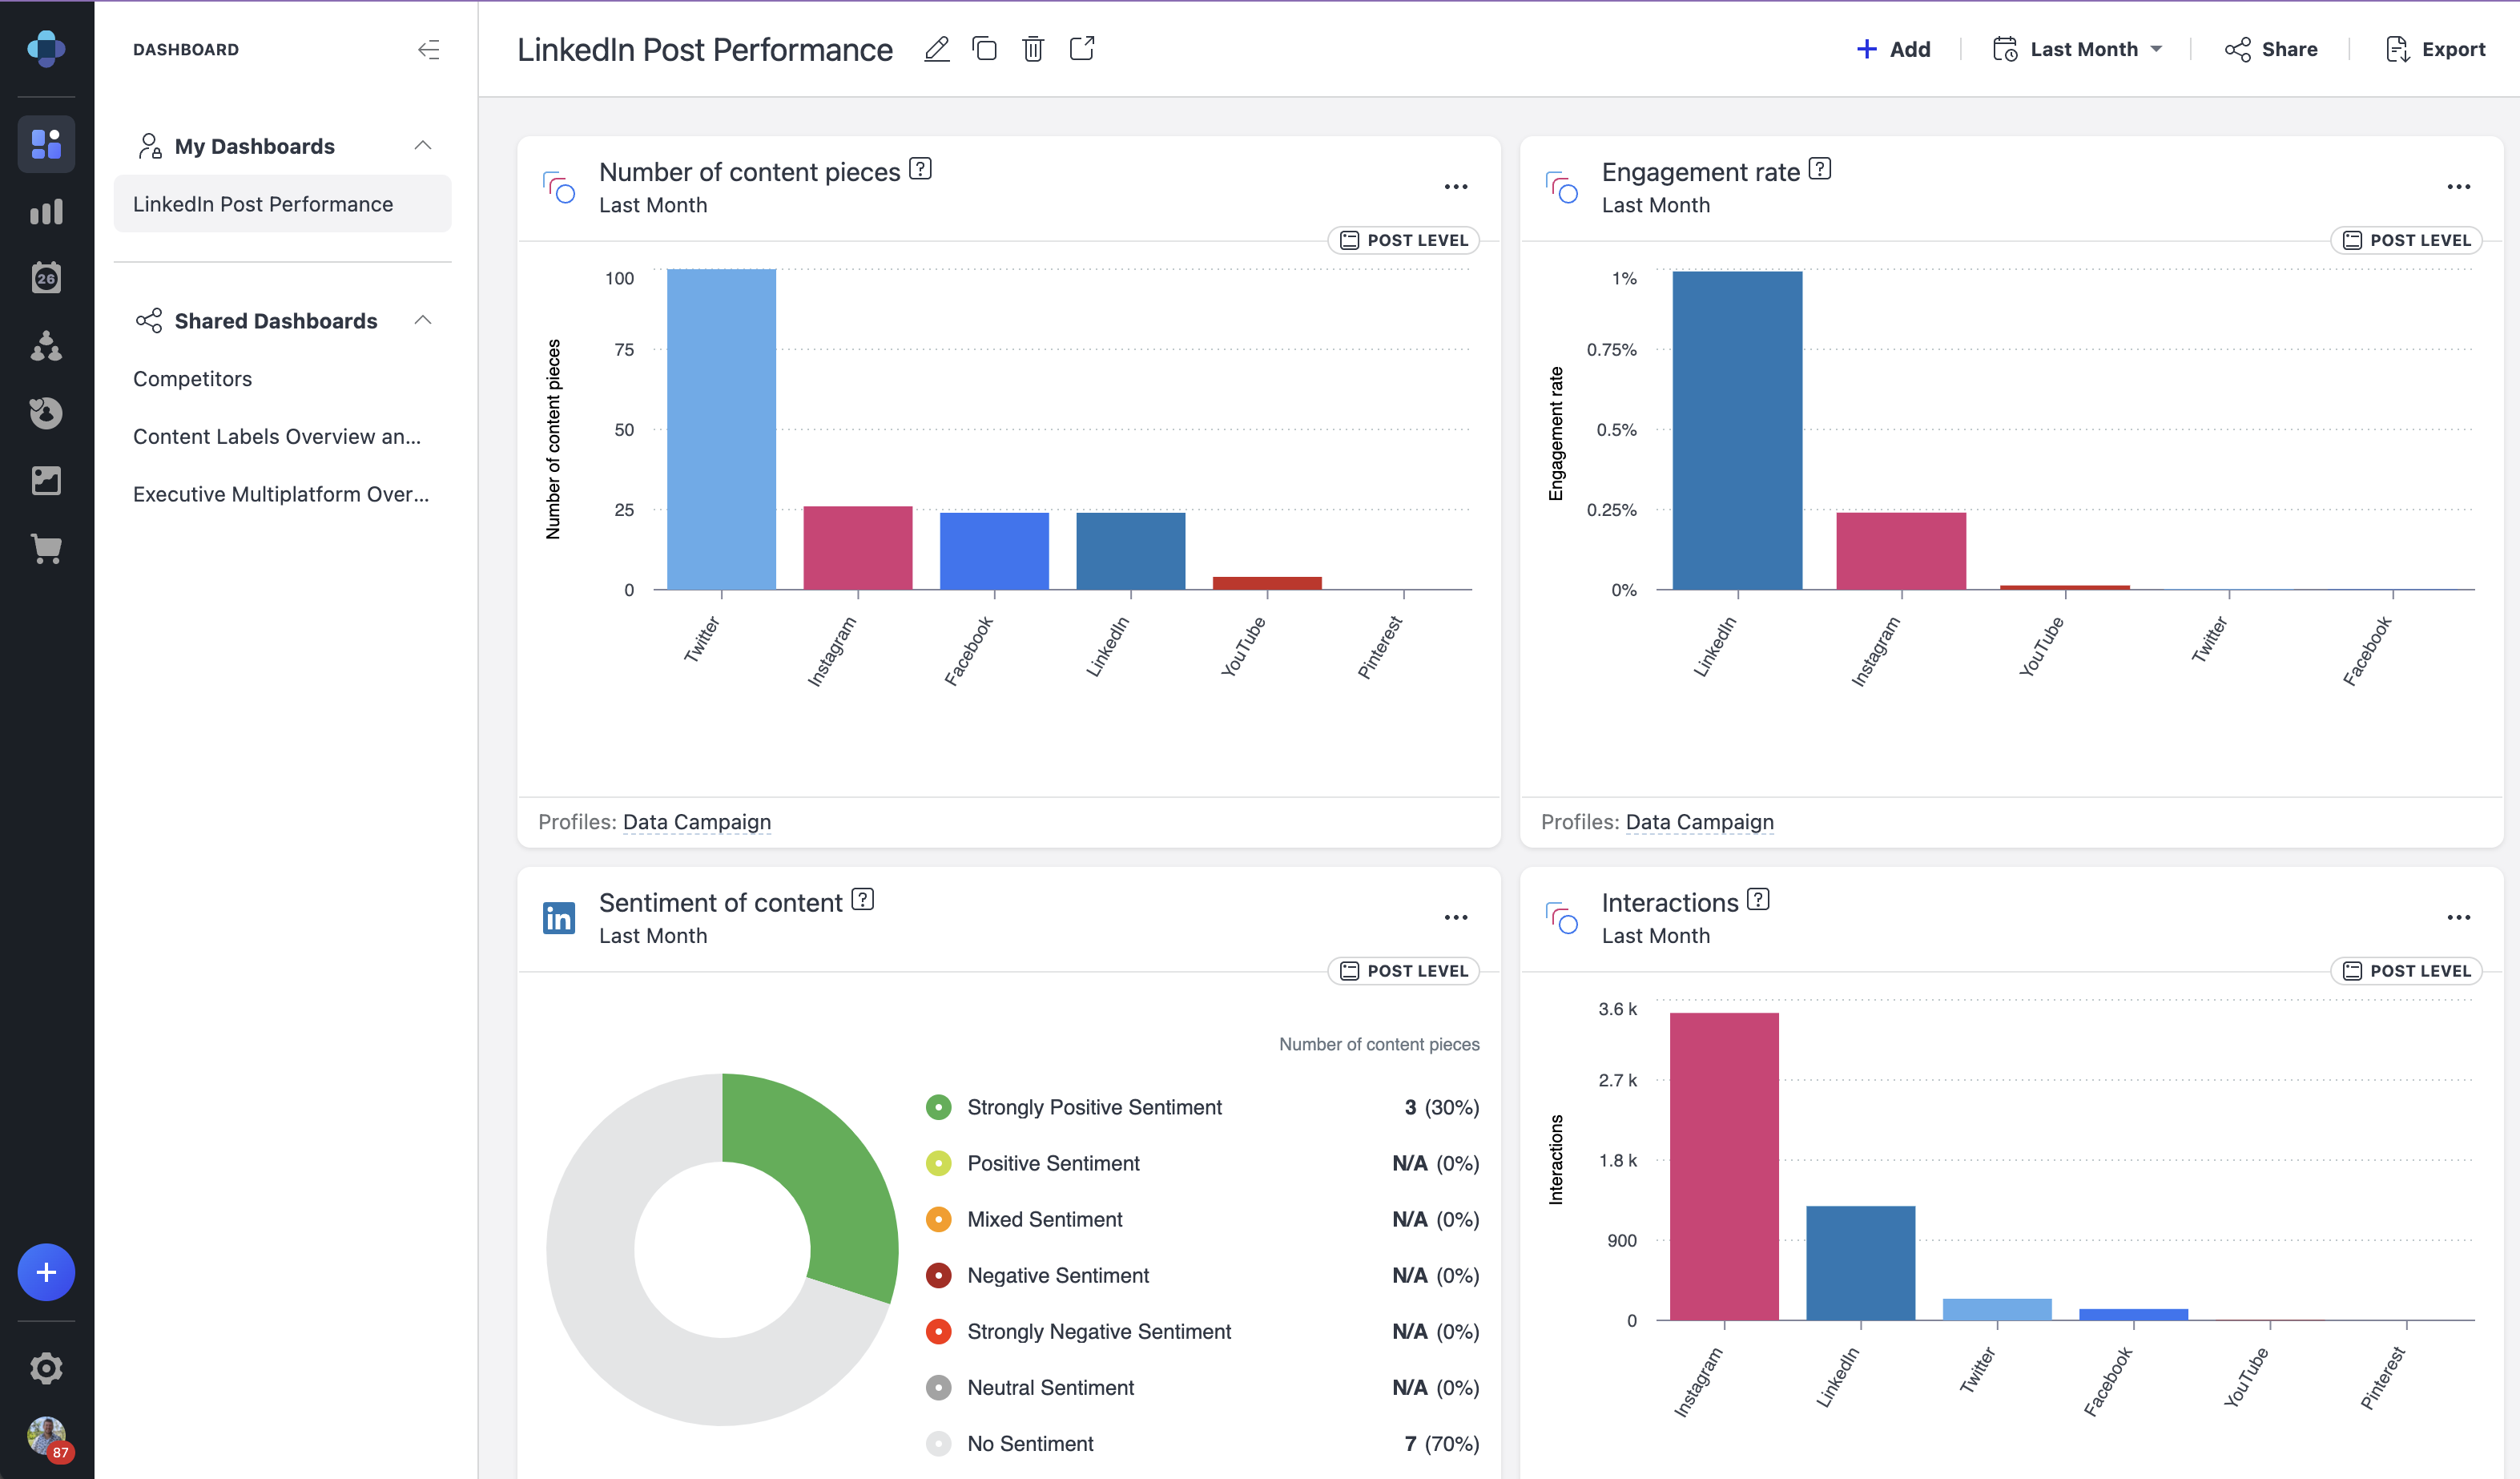
\includegraphics[width=1\textwidth]{pictures/emplifi-dashboard-example.png}
	\caption{Ukázka dashboardu v produktu firmy Emplifi \cite{emplifidashboardIMAGE}}
	\label{fig:emplifiDashUkazka}
\end{figure}

Na obrázku \ref{fig:emplifiDashUkazka} vidíme příklad dashboardu - skládá se z několika grafů, obvykle nazývané jako widgety \cite{emplifiDashboard}, jejichž obsah lze modifikovat pomocí přepínačů v liště. Obsah může být modifikován v časovém období (posledních 30 dní, poslední rok, konkrétní časový rozsah, ...), ale lze jej modifikovat také na základě metrik jako je např. sociální síť (Facebook, Instragram, LinkedIn), druh interakcí (komentáře, liky, sdílení) apod.\footnote{Widgety nemusí být obecně pouze vizualizace, může se jednat také o ovládací prvky (např. výběrové seznamy, check boxy, textfieldy apod.). Tato možnost se využívá zejména ve vývojářských dashboardech pro rychlejší tvorbu vizualizací. V samotném produktu firmy se ale používá kvůli uživatelské přívětivosti pouze pro vizualizace \cite{emplifiDashboard}. 
}

Embedded analytics se nechová a nevypadá jako samostatná aplikace, ale je integrován do jiného softwaru nebo webového portálu. Koncoví uživatelé často ani nepoznají, že se jedná
integrovanou analytiku a vnímají software s touto integrovanou analytikou jako jeden nástroj \cite{goodDataEmbedded}. To umožňuje softwarovým společnostem získat a plně
integrovat analytickou platformu s jejich vlastním SaaS produktem bez nutnosti velkých investic do vývoje vlastního řešení. 

SaaS (Software as a Service) je licenční model, v němž přístup je poskytován na základě předplatného, přičemž software je umístěn na externích serverech, nikoli na firemních serverech \cite{saasDefinition}.
K těmto službám se běžně přistupuje prostřednictvím webového prohlížeče s přihlašovacím jménem a heslem. Výhodou je, že místo toho, aby mělo každé zařízení ve firmě nainstalované
tento program, stačí se do programu přihlásit přes internet. Pro firmu to znamená úsporu financí, jelikož nemusí investovat do nového hardwaru, na němž by dané programy běžely. 
Nevýhodou SaaS je bezpečnost dat a rychlost jejich doručování. Protože jsou data umístěna na externích serverech, je třeba zajistit rychlé a spolehlivé internetové připojení a vyloučit
přístup neoprávněných uživatelů.

Existuje hned několik způsobů, jak data embedovat. Mezi nejpopulárnější a nejrozšířenější způsoby patří HTML iframe, webová komponenta či React SDK s voláním API \cite{goodDataEmbedded}. 

\subsection{Iframe}
Nejjednodušší a nejrychlejší metodou embedování je využití použití iframu \cite{goodDataEmbedded}. Iframe (inline frame) je HTML prvek, který umožňuje načíst HTML stránku uvnitř dokumentu \cite{iFrameAdv}. Používá se pro vložení určitého obsahu z jednoho zdroje do druhého. To se poté jeví jako nové okno v dané stránce, jedná se ovšem o embedovaný iframe. Tuto možnost embedování využívají např. Google Mapy nebo YouTube \cite{iFrameAdv}. Velkou výhodou je, že není třeba instalovat pro běh žádné dependence.

\subsection{Webová komponenta}
Pokročilejší technikou pro embedování je použití webové komponenty. Výhoda opět spočívá v tom, že není třeba instalovat závislosti pro běh. Embedování probíhá pomocí knihovny, která se naimportuje přes HTML tag \texttt{<script>}. Poté je možno embedovat vizualizace pouze prostřednictvím naimplementovaných webových komponent \cite{webComp}.

\subsection{React SDK + API}
Poslední zmiňovanou možností je embedování prostřednictvím React SDK s voláním API. 

SDK (Software development kit) je označení sady nástrojů pro tvorbu softwaru \cite{SDKvsAPI}, které umožňuje vývojářům vytvářet rychleji a standartizovaně nové aplikace. API 
(Application Programming Interface) je rozhraní usnadňující komunikaci mezi dvěmi platformami. Uživatel specifikuje požadavek na data, rozhraní API provede volání na webový server, který
následně tento požadavek zpracuje a odešle odpověď na specifikované volání (může se jednat např. o data ve formátu JSON). Díky tomu se krátí vývojový cyklus (automatizace), efektivně 
se poskytují nové služby uživatelům a může zlepšit reputaci důvěryhodnost značky.

K embedování je potřeba následovat instrukce (např. nainstalování dependencí, zprovoznění backendu apod.) a zajistit, že všechny kroky v nich obsažené budou splněny \cite{reactSDKComp}. Jedná se tedy o programátorsky náročnější metodu, ovšem výhoda spočívá ve větší flexibilitě vývojářů, kteří mohou vizualizace snadno modifikovat \cite{goodDataEmbedded}.

%
% Podkapitola zabezpečení
%
\section{Zabezpečení}
Zabezpečení API je důležitou součástí v moderním inženýrství zajišťující bezpečnou a důvěryhodnou komunikaci mezi různými aplikacemi. S rostoucím významem API pro výměnu dat mezi
systémy je nezbytné věnovat zvláštní pozornost implementaci efektivních bezpečnostních opatření. API authentication (autentizace) je řešením pro ověřování uživatelů - to umožňuje
vlastníkovi daného API ochranu před neoprávněným přístupem ze strany uživatelů, kteří nemohou ověřit svou totožnost \cite{whatIsAPI}.

Řešení autentizace jsou obvykle nastavena tak, aby zablokovala přístup do API, pokud se při volání zjistí něco nesprávného či nevalidního s uživatelem. S tím se pojí druhá bezpečnostní
složka, kterou je autorizace (authorization). Zatímco autentizace ověřuje identitu uživatele, autorizace se zabývá tím, jaké akce má daný uživatel povoleny \cite{mostUsedAuthentication}. 
Mezi nejpoužívanější metody patří HTTP authentication, API keys a OAuth 2.0. 

\subsection{HTTP autentizace}
HTTP autentizace omezuje přístup k serveru pomocí předdefinovaných schémat. 

Jedním z používaných schémat je Basic HTTP \cite{mozillaHTTPAuth}. Uživatel, který chce ověřit svou identitu, tak může učinit vložením hlavičky 
Authorization s bezpečnostními údaji - nejčasteji tím bývá uživatelské jméno a heslo. 
Samotné ověřování pomocí HTTP Basic se ovšem nedoporučuje. Přenášené údaje jsou sice zakódované, ale nejsou zašifrované \cite{mozillaHTTPAuth}. Proto je třeba v případě použití zajistit šifrované spojení (HTTPS/TLS). Atribut hlavičky se zakódovaným uživatelským jménem a heslem může vypadat např. jako na ukázce \ref{basicHeader}.

\begin{lstlisting}[language=json, caption={Autorizační atribut - Basic schéma}, label=basicHeader]
	Authorization: Basic drgnpdrgud653==,
\end{lstlisting}

Bearer schéma obsahuje tzv. bearer tokeny. Bearer token specifikuje, k jakým zdrojům může uživatel v API přistupovat \cite{mostUsedAuthentication}. Token je obvykle řetězec vygenerovaný serverem v reakci na požadavek na přihlášení. Opět je nutné zajistit zabezpečené spojení jako v případě Basic schématu. Atribut hlavičky s tokenem může vypadat např. jako na ukázce \ref{bearerHeader}

\begin{lstlisting}[language=json, caption={Autorizační atribut - Bearer schéma}, label=bearerHeader]
	Authorization: Bearer se5Edg345dsBNN-7df,
\end{lstlisting}


\subsection{API key}
API klíč (key) je jedinečný alfanumerický řetězec, který slouží k jednoznačné identifikaci klientů/aplikací \cite{amazonAPIKey}, jenž API využívají. Narozdíl od tokenů
nejsou časově omezené - to může znamenat bezpečnostní problém v případě, že při zadávání požadavku API by přenášený klíč mohl být zachycen \cite{mostUsedAuthentication} a s ním i celá síť, pokud by obsahovala jeden nezabezpečený bod. Proto je i v tomto případě nutné zajistit šifrované spojení \cite{keepingApiKeysSafe}.
Pokud API bude sloužit pouze ke čtení, je zabezpečení API klíčem tou nejlepší volbou - uživatelé budou moci data stahovat, ale nikterak modifikovat či mazat \cite{mostUsedAuthentication}. 

\subsection{OAuth}
OAuth (Open Authorization) protokol byl vyvinut jako řešení pro udělování přístupu na předem definovanou dobu bez sdílené uživatelských jmen a hesel \cite{understandingOAuth2}. OAuth 2.0
je nejlepší volbou pro identifikaci osobních uživatelských účtů a udělování patřičných oprávnění \cite{mostUsedAuthentication}. Proces autentizace je vidět na obrázku \ref{fig:oauth2Diagram}.


\begin{figure}
	\centering
	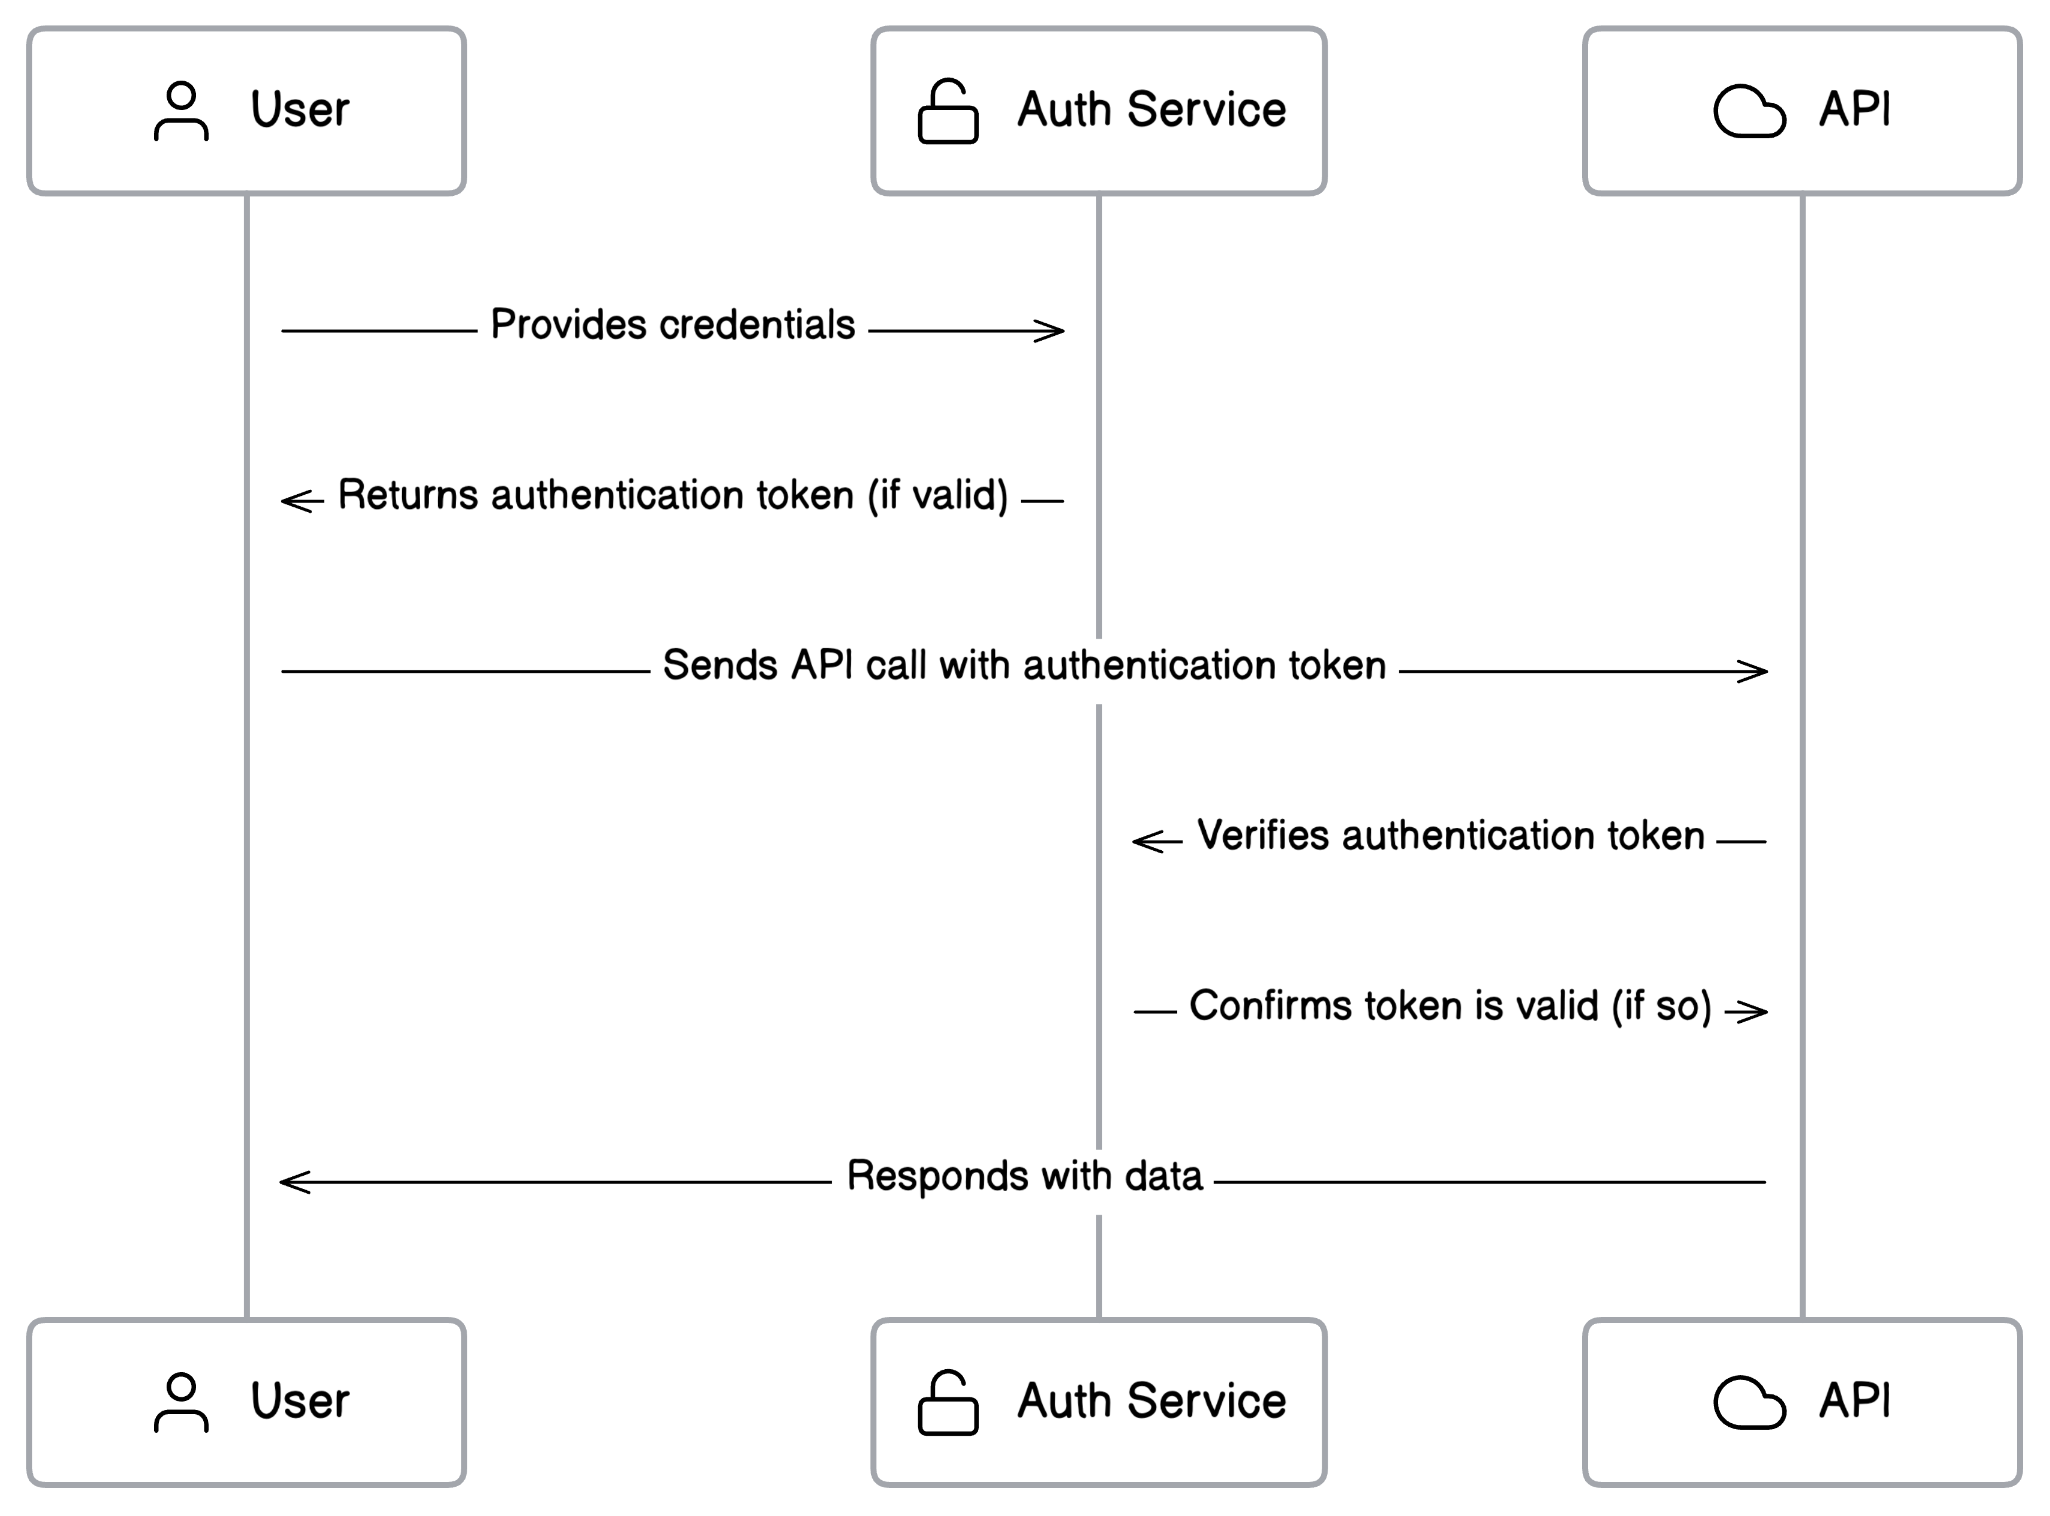
\includegraphics[width=1\textwidth]{pictures/oauth2-diagram.png}
	\caption{Autentizační diagram protokolu OAuth 2.0 \cite{oAuthImage}}
	\label{fig:oauth2Diagram}
\end{figure}


Nejprve se uživatel přihlásí do systému - nejčastěji formou uživatelského jména a hesla, nebo klientského id a secretu. Tím se pošle HTTP požadavek na endpoint. Autorizace uživateli následně
vrátí token. Pokud má uživatel již platný token, může přistupovat k datům. Naopak pokud mu token již expiroval nebo není platný, volání do API mu vrátí chybové hlášení. 

Součástí autorizační odpovědi bývá i několik dalších údajů. Odpověď může vypadat např. jako na \ref{tokenResponse}. 

\begin{lstlisting}[language=json, caption={Ukázková odpověď autorizačního serveru}, label=tokenResponse]
{
	"access_token": "G7k4Q2s1bD5z9x",
	"token_type": "Bearer",
	"expires_in": 3600,
	"refresh_token": "5aB3c9Cx8P5y2z",
	"scope": "create"
}
\end{lstlisting}
	  
Odpověď bývá ve formátu JSON (JavaScript Object Notation) a obsahuje informace o daném přístupovém tokenu (access\_token). Kromě přístupového tokenu obvykle obsahuje i refresh\_token. Ten umožňuje uživateli 
používat stále jeden token bez nutnosti generování nového \cite{oauthResponseExample}. Dále může obsahovat specifikující práva uživatele (scope), platnost tokenu (expires\_in) či typ tokenu (token\_type), jež některé z nich byly zmíněny v předchozí kapitole.
Přesný formát odpovědi je ale specifikován samotným API - tudíž každé API může mít jiné délky přístupových a obnovovacích tokenů, časové platnosti tokenů či i samotné atributy v odpovědi a jejich názvy.
%
% Podkapitola existující řešení
%
\section{Existující řešení}
Embedded analytics problematikou se zabývá mnoho firem a každá z nich disponuje jinými způsoby řešení. Zde budou zmíněny firmy, které se objevují často na vrchních příčkách
internetových recenzí či firmy, které byly pro inspiraci doporučeny externím zadavatelem. Pro aktuálnost jsou brány informace ze zdrojů z roků 2022/2023.
\subsection{GoodData}
Firma GoodData byla zmíněna zadavatelem jako jedna z nejvýraznějších na trhu. Dodává embedded analytics systémy firmám jako je VISA, Zalando či Bentley \cite{goodDataEmbeddingPlatform}. 
Embedování provádí třemi zmíněnými způsoby - HTML iframem, webovou komponentou či React SDK. Zákazníkům nabízí přizpůsobení dashboardů tak, aby odpovídaly zákazníkovo značce. GoodData získaly
v roce 2023 hned několik ocenění firmou TrustRadius, důvěryhodnou platformou v oblasti B2B (bussines to bussines) \cite{trustRadiusDiscusionGoodData}. Firma GoodData obdržela ocenění Best Value for Price,
Best Relationship či Top Rated 2023. Zákazníci firmy GoodData si v recenzích chválí hlavně snadné používání, zákaznickou podporu, širokou škálu podporovaných databází či uživatelsky přívětivé
rozhraní \cite{trustRadiusDiscusionGoodData}. Naopak se zmiňují, že dokumentace může být nedostačující či některé endpointy v API mají neintuitivní parametry. I tak ale 92\% recenzentů uvádí,
že by si produkt zakoupili znovu.

\subsection{Microsoft Power BI}
Mezi často zmiňovaným produktem je Microsoft Power BI, který je ve svém oboru nejlepší v oblasti bezpečnosti a zabezpečení \cite{bestEmbTools2023},
jelikož Microsoft zaměstnává více než 3500 bezpečnostních expertů. V produktu nabízí také tzv. playground, který
umožňuje uživatelům testovat funkce a vlastnosti daných dashboardů před úplným nasazením. Je také podporvána integrace s cloudovou službou Microsoft Azure. Na webu TrustRadius je k 
Microsoft Power BI podstatně méně recenzí než k produktu GoodData (5x méně). Uživatelé zmiňují dlouhou dobu při zpracování většího objemu dat či vysokou provozní cenu \cite{trustRadiusDiscusionAzure}.

\subsection{Powered by Looker}
V oblasti modelování data vyniká platforma Powered by Looker \cite{bestEmbTools2023}. Jedná se o produkt služby Google Cloud, který poskytuje způsob, jak sledovat změny a prohlížet jejich
historii v databázi. Disponuje modelovacím jazykem LookML založeným na SQL, který slouží k vytváření sémantických datových modelů. Pomocí něj lze popisovat jednotlivé dimenze, agregáty,
výpočty či datové vztahy v databázi \cite{googleLookMLDoc}. Z toho vyplývá, že datové modely jsou rozšiřitelné, opakovatelně použitelné a konzistentní a tudíž efektivní. V roce 2022 byl tento produkt
oceněn Top Rated a Most Loved společností TrustRadius \cite{trustRadiusDiscusionLooker}. Uživatelé zmiňují, že produkt může být pomalejší a že nástroje na přizpůsobení dashboardů by mohly být
vylepšeny a rozšířeny.


\subsection{Tableau}
Tableau vyniká ve vytváření estetických a interaktivních vizualizací \cite{tableauBlog}. Dále nabízí zákazníkům publikaci vizualizací prostřednictvím produktu Tableau Online. Cena produktu začíná na \$70 měsíčně za jednoho uživatele \cite{trustRadiusTableAU}. 
Zákazníci produkt hodnotí velmi kladně - 100\% z nich uvádí, že implementace proběhla jak očekávali, 98\% jsou s výsledkem spokojeni a 91\% by si tento produkt zakoupilo zase \cite{trustRadiusTableAU}. Silné stránky 
tohoto produktu spočívají v automatickém generování kódu pro embedování a jednoduché vkládání dashboardů do webových stránek \cite{tableauBlog}. Kritika naopak zaznívá na zákaznickou podporu či pomalé načítání při velkém množství dat \cite{trustRadiusTableAU}.

% _____________________________________________________________________________
%
%
%        CHAPTER Návrh knihovny
%
% _____________________________________________________________________________
%
\chapter{Návrh knihovny a uživatelského rozhraní}

V této kapitole bude popsán detailní návrh knihovny, uživatelského rozhraní a technologie, jež budou použité k realizaci. 

\section{Technologie}

\subsection{JavaScript a React}
Pro vývoj knihovny bude využit JavaScript s knihovnou React. Důvodem zvolení těchto technologií je požadavek ze strany zadavatele. React a JavaScript jsou dnes
široce používané technologie ve vývoji webových aplikací. 

React je snadný na naučení, obsahuje málo konceptů, které je třeba se naučit \cite{whyUsingReact}. Jeho instalace je snadná -
stačí pouze v kódu nainstalovat a naimportovat jeho knihovnu. Využívá speciální JSX syntaxe, která sice vypadá jako HTML, ale ve skutečnosti je tato syntaxe převáděna na HTML. Jelikož je React hojně využíván
v aplikaci Facebook či na Instagramu, dostává se mu velké podpory právě i z tohoto odvětví - čtyři největší přispěvatelé knihovny React jsou zaměstnanci Facebooku \cite{whyUsingReact}. Kromě 
Facebooku využívají React značky jako jsou např. Netflix, airbnb, BBC News či PayPal \cite{whyUsingReact2}. Díky virtualizaci a uchováváním DOM poskytuje React
velmi rychlé vykreslování, přičemž všechny změny se snadno promítají do virtuálního DOM. 

DOM (Document Object Model) je strukturovaná reprezentace jazyka HTML, které reprezentuje celé uživatelské rozhraní jako stromovou datovou strukturu \cite{whatIsDOM}. Každý prvek uživatelského
rozhraní tvoří v DOM stromu právě jeden uzel. Dojde-li ke změně uživatelského rozhraní, DOM se aktualizuje 	a při každé změně se vykresluje znovu, což výrazně ovlivňuje výkon aplikace. 
Toto lze vyřešit použitím virtuálního DOM. Při přidávání nových věcí do aplikace se vytvoří virtuální DOM, která je reprezentován jako strom. Novější virtuální DOM se porovnává se starším, aby
zaznamenal změny. Poté zjistí, jak je možné tyto změny provést pomocí skutečného DOM a aktualizované prvky se následně vykreslí.

React využívá tzv. komponent, které slouží k vizualizaci aplikace \cite{introToReact}. Existují dva druhy těchto komponent - funkcionální a třídní \cite{functionalVsClass}. Knihovna bude používat funkcionální, jelikož
se jedná o novější verzi komponent.

Na popularitě Reactu přidává také použití knihovny Redux, která umožňuje uchování dat jako jeden objekt (stav). Použití Reduxu je vhodné zejména u velkých aplikací - čím větší je aplikace, tím
náročnější je správa stavu aplikace \cite{introToRedux}. K reduxovému stavu objektu se dá pak jednoduše přistupovat, což značně usnadňuje práci s daty.
Je-li tento stav změněn, aplikace se překreslí a zobrazení se stále synchronizuje se souvisejícími daty \cite{whyUsingReact2}. 

React se kvůli těmto vlastnostem doporučuje využívat u:
\begin{enumerate}
\item Obsáhlých uživatelských rozhraní
\item Rozsáhlých aplikací
\item Aplikací náročné na výkon
\item Multi-platformních aplikací
\end{enumerate}

Na frontend komponent knihovny a rozhraní pro obnovu tokenů bude použita knihovna MUI, která nabízí širokou škálu předdefinovaných komponent a stylů \cite{muiDocs}. 	

\subsection{Emplifi API}	
Data potřebná k embedování grafů budou získávána prostřednictvím Emplifi Public API. 
Toto rozhraní poskytuje klientům snadný a oblíbený způsob, jak získat přístup k potřebným datům. 
Emplifi API se nachází na veřejné webové adrese a žádat o data může každý, kdo má přístupový token.
Struktura dotazů a ukázkové dotazy jsou dostupné na veřejné dokumentaci \cite{emplifiDocs}.

\subsubsection{Vytvoření tokenu}

Vytvoření tokenu je umožněno pouze osobám, jež mají u firmy Emplifi vytvořený účet v produktu Suite. Na diagramu \ref{fig:emplifAPIDiagram} je schéma, které udává průběh akcí během žádání o 
přístupový token a zaslání prvního requestu s žádostí o data.
\begin{figure}
	\centering
	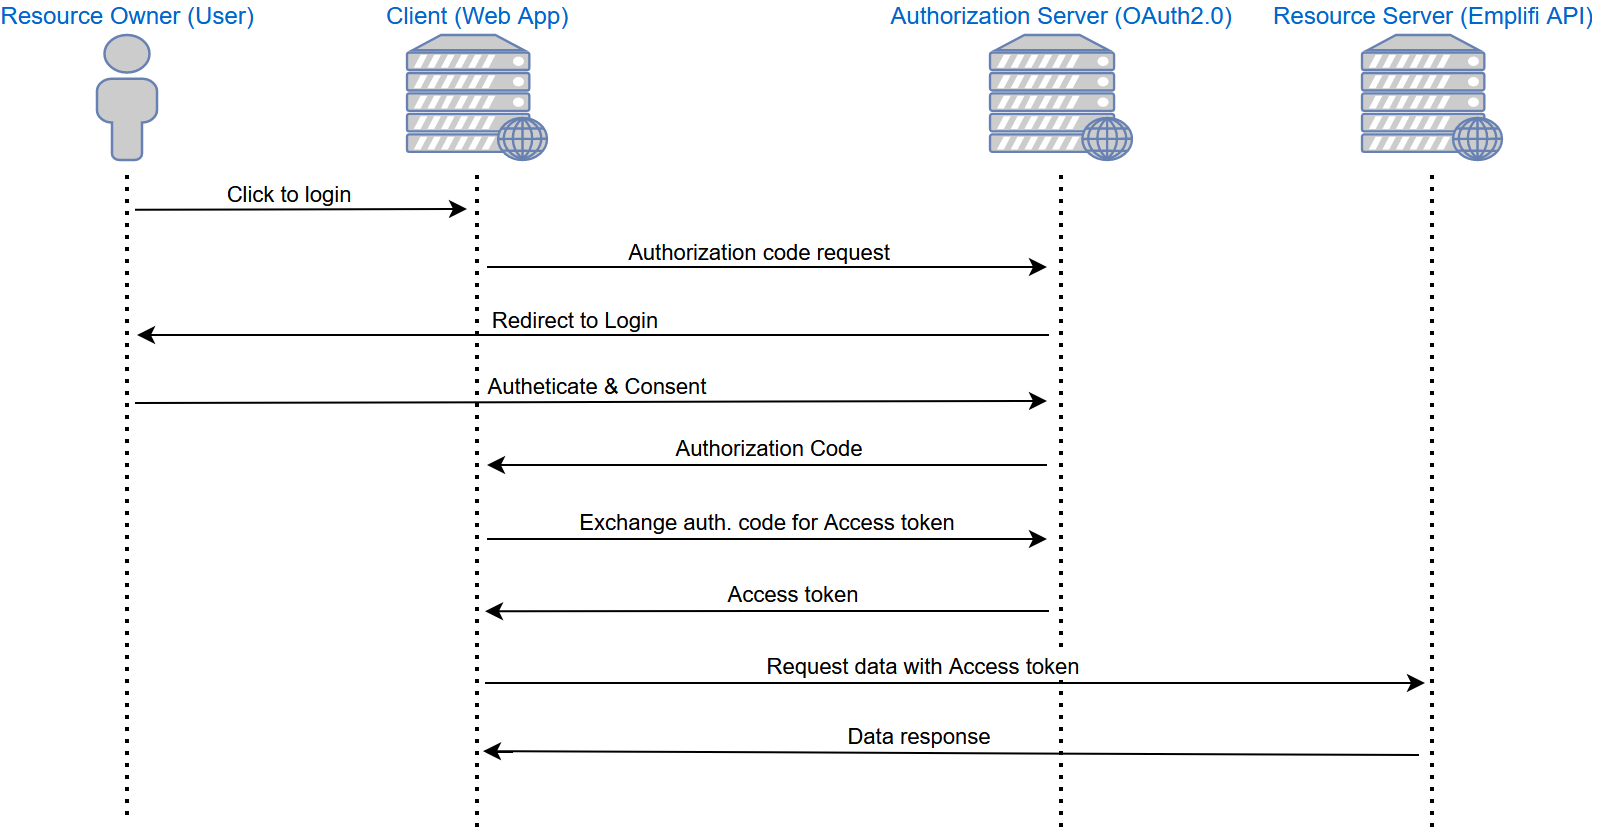
\includegraphics[width=1\textwidth]{pictures/emplifiAPI.png}
	\caption{Diagram vytvoření Emplifi API tokenu \cite{emplifiDocs}}
	\label{fig:emplifAPIDiagram}
\end{figure}

Pro vytvoření tokenu je třeba uživatele přesměrovat na webovou URL \url{https://api.emplifi.io/oauth2/0/auth}, kde bude požádán o udělení souhlasu z jeho Emplifi Suite účtu.
Do URL, na kterou uživatele přesměrujeme, bude třeba vložit několik parametrů potřebných k autentizaci a k následnému vrácení tokenu. 

\begin{center}
	\begin{longtable}{p{.2\textwidth}p{.65\textwidth}}
	\caption{Seznam všech parametrů vkládaných do URL adresy při tvorbě tokenu \cite{emplifiDocs}}
	\label{tab:allParametersAPI}\\
	\toprule[1.5pt]
	\endhead
	\midrule
	\multicolumn{2}{r}{\textit{(tabulka pokračuje na další stránce)}}\\
	\endfoot
	\bottomrule[1.5pt]
	\endlastfoot
	%
	\verb"client_id" &  Jedinečný klientský identifikátor pro aplikaci.\\
	\midrule
	\verb"redirect_uri" & Návratová adresa. Na tuto adresu bude při úspěšné autorizaci přesměrován přístupový token. Zároveň tato adresa musí být povolena vývojáři v interní databázi.\\
	\midrule
	\verb"response_type" & Typ - Emplifi momentálně podporuje pouze hodnotu "code".\\
	\midrule
	\verb"scope" & Specifikuje prostředky oddělené mezerou, ke kterým aplikace může přistupovat klientským účtem. Ty při udělování souhlasu budou předloženy ke schválení. \\
	\midrule
	\verb"state" & Hodnota sloužící k validaci přijaté odpovědi. Při zaslání requestu je vložena hodnota do parametru, autorizační server jí při zpracování dotazu odešle zpět s daty. Uživatelská aplikace by následně měla porovnávat, zda tato zaslaná hodnota je shodná s původní - to slouží k zabránění útoků Cross-site Request Forgery.\\
	\midrule
	\verb"prompt" & Musí být nastavena na hodnotu "consent", pokud má být refresh token vrácen společně s přístupovým.\\
	\end{longtable}
\end{center}


Pokud veškeré parametry budou správně nastaveny a uživatel udělí souhlas s používáním Suite účtu, na URL \texttt{redirect\_uri} se vrátí zpráva s autorizačním kódem. Tento kód
slouží k výměně za přístupový token. O ten je možno si zažádat POST requestem na adresu \url{https://api.emplifi.io/oauth2/0/token}. Struktura requestu je popsána v tabulkách \ref{tab:exampleRequestHeader} a \ref{tab:exampleRequestBody}.

\begin{center}
	\begin{longtable}{p{.2\textwidth}p{.65\textwidth}}
	\caption{Hlavička requestu na token \cite{emplifiDocs}.}
	\label{tab:exampleRequestHeader}\\
	\toprule[1.5pt]
	\endhead
	\midrule
	\multicolumn{2}{r}{\textit{(tabulka pokračuje na další stránce)}}\\
	\endfoot
	\bottomrule[1.5pt]
	\endlastfoot
	%
	\verb"Authorization" & Řetězec "Basic" s klientským identifikátorem a zakódovaným klientským secretem oddělený dvojtečkou v Base64. Výsledná hodnota vypadá např. takto: "Basic Y2xpZW50X2lkOmNsaWVudF9zZWNyZXQ=."\\
	\midrule
	\verb"Content-Type" & Hodnota "application/x-www-form-urlencoded" \\
	\end{longtable}
\end{center}

\begin{center}
	\begin{longtable}{p{.2\textwidth}p{.65\textwidth}}
	\caption{Tělo requestu na token \cite{emplifiDocs}.}
	\label{tab:exampleRequestBody}\\
	\toprule[1.5pt]
	\endhead
	\midrule
	\multicolumn{2}{r}{\textit{(tabulka pokračuje na další stránce)}}\\
	\endfoot
	\bottomrule[1.5pt]
	\endlastfoot
	%
	\verb"code" & Řetězec sloužící k následné validaci při zpětném volání. \\
	\midrule
	\verb"grant_type" & Hodnota "authorization\_code" \\
	\midrule
	\verb"redirect_uri" & URL adresa, kam bude přesměrován token. Musí být stejná jako v tabulce \ref{tab:allParametersAPI} \\
	\end{longtable}
\end{center}

Následně obdržíme token ve formátu jako na \ref{tokenResponse}. Přesné návratové hodnoty jsou popsány v tabulce \ref{tab:exampleRequestResponse}.

\begin{center}
	\begin{longtable}{p{.2\textwidth}p{.65\textwidth}}
	\caption{Tělo odpovědi se zaslaným tokenem \cite{emplifiDocs}.}
	\label{tab:exampleRequestResponse}\\
	\toprule[1.5pt]
	\endhead
	\midrule
	\multicolumn{2}{r}{\textit{(tabulka pokračuje na další stránce)}}\\
	\endfoot
	\bottomrule[1.5pt]
	\endlastfoot
	%
	\verb"access_token" & Přístupový token k Emplifi Public API. \\
	\midrule
	\verb"token_type" & Jediný podporovaný typem je "bearer". \\
	\midrule
	\verb"expires_in" & Platnost tokenu ve vteřinách. \\
	\midrule
	\verb"refresh_token" & Token pro obnovení přístupového tokenu. Zaslán pouze v případě, pokud \verb"scope" obsahuje řetězec "offline\_access".\\
	\midrule
	\verb"scope" & Prostředky, které byly uživatelem uděleny. Odděleny mezerou. \\
	\end{longtable}
\end{center}



Užívání tokenů má ovšem nastavené limity - 500 requestů za hodinu pro uživatele, 1000 requestů za hodinu pro účet \cite{emplifiDocs}. Pokud bude tato hranice přesažena,
API vrátí odpověď s informací, že uživatel či účet překročili maximální limit dotazů.

\subsubsection{Endpointy}

Má-li uživatel platný token, může začít se zasíláním dotazů. Emplifi API disponuje množstvím endpointů, přičemž endpointy využívané k embedování jsou zmíněné v tabulce \ref{tab:embeddingEndpoints}. 

\begin{center}
	\begin{longtable}{p{.25\textwidth}p{.6\textwidth}}
	\caption{Endpointy používané k embedování.}
	\label{tab:embeddingEndpoints}\\
	\toprule[1.5pt]
	\endhead
	\midrule
	\multicolumn{2}{r}{\textit{(tabulka pokračuje na další stránce)}}\\
	\endfoot
	\bottomrule[1.5pt]
	\endlastfoot
	%
	\verb"/3/omni/metrics" & Získávání dat pro vizualizace. Data jsou ve formátu omni. \\
	\midrule
	\verb"/3/omni-studio" &  Získávání widget konfigurací, fieldů a vytváření Omni API tokenů\\
	\midrule
	\verb"/oauth2/0" &  Vytváření Public API tokenů. \\
	\end{longtable}
\end{center}

Endpoint omni-studio bylo nutné vytvořit zadavatelem, jelikož Omni API endpointy bylo možné volat pouze při použití firemní VPN (Virtual Private Network). Nyní lze tyto endpointy provolávat prostřednictvím Public API. Původní
strukturu Omni API requestu lze vložit do těla public API requestu, což umožní uživateli embedovat grafy i mimo VPN.

\subsubsection{Knihovny pro fetchování dat}

V současné době existuje mnoho knihoven určené pro fetchování dat. Data bude nejprve nutné načíst na backend běžící aplikace, která je následně vrátí na frontend. Na backendu probíhá fetchování dvojím způsobem - 
využitím zabudovaného fetch API v Node.js a knihovnou axios. Pro načítání dat z backendu na frontend budeme využívat rozhraní JavaScriptu Fetch API a knihovnu TanStack React Query. Její výhodou je cachování
requestů \cite{tanstackQueryDocs} - pokud byl poslán jednou již stejný dotaz na data, načtení dat neproběhne z API, ale z uložené cache. To omezí počet requestů zaslaných na API a zmenší prodlevu vizualizace (data načtou rychleji z cache než z API). 

\subsection{PreJSON a Vision}

Interní knihovny, které budou využiti k upravování widget konfigurací (PreJSON) a následné vizualizaci grafů (Vision).

PreJSON slouží k expandování konfigurací widgetů. Stažené konfigurace widgetů obsahují tzv. preJSON hodnoty, které jsou později dodefinovány uživatelem. Např. je-li stažena konfigurace, která obsahuje
nespecifikovaný parametr, můžeme jej dodefinovat použitím instance PreJSONu \cite{preJSONDocs}. Na zjedodušené ukázce \ref{notExpandedPreJson} je zobrazen PreJSON objekt, který by mohl specifikovat tělo dotazu. 

\begin{lstlisting}[language=json, caption={Neexpandovaný PreJSON objekt}, label=notExpandedPreJson]
{
	customer_id: 12651141417427,
	time: "P30D/now[sD]",
	platform: ${string:platform_name}
}
\end{lstlisting}
		
Atributy \texttt{customer\_id} a \texttt{time} jsou již předdefinové, ale na uživateli zůstává možnost volby parametru \texttt{platform}. Datový typ parametru musí být vždy specifikován.
Zde se očekává string hodnota, která může nabývat (opět pouze pro ukázku) např. hodnot "instragram", "facebook", "snapchat", "linkedin" apod. Uživatel tedy zvolí jednu ze sociálních sítí
a pomocí funkce \texttt{expand()} může tuto hodnotu dodefinovat. Výsledek může vypadat poté jako na ukázce \ref{expandedPreJson}.

\begin{lstlisting}[language=json, caption={Expandovaný PreJSON objekt}, label=expandedPreJson]
{
	customer_id: 12651141417427,
	time: "P30D/now[sD]",
	platform: "snapchat"
}
\end{lstlisting}

Knihovna Vision slouží k vytváření vizualizací. Obsahuje komponentu, která ovšem nespecifikuje, jak daná vizualizace bude vypadat \cite{visionDocs}, ale slouží k vykreslení vizualizace. 
Veškeré data a konfigy vizualizace (např. jakou barvu bude mít graf, jaká je popsána osa X apod.) jsou předány uživatelem a knihovna se pouze postará o vykreslení. Tato výsledná vizualizace 
neobsahuje ale např. nadpisy, nápovědy apod., to bude zajišťovat výsledná knihovna této bakalářské práce.

O vykreslování se stará komponenta \texttt{<Vision/>}. Pro potřeby BP budou využívány parametry uvedené v tabulce \ref{tab:visionParams}.

\begin{center}
	\begin{longtable}{p{.2\textwidth}p{.65\textwidth}}
	\caption{Parametry komponenty <Vision/>}
	\label{tab:visionParams}\\
	\toprule[1.5pt]
	\endhead
	\midrule
	\multicolumn{2}{r}{\textit{(tabulka pokračuje na další stránce)}}\\
	\endfoot
	\bottomrule[1.5pt]
	\endlastfoot
	%
	\verb"spec" & Validní JSON expandovaná konfigurace grafu (druh grafu, popisky os, barvy grafu apod.). \\
	\midrule
	\verb"input" &  Data zobrazována v grafu. \\
	\end{longtable}
\end{center}

Následně je třeba tuto komponentu s předanými parametry vložit do komponenty \texttt{<VisionContextProvider/>}, aby došlo ke správnému vyrenderování.

\section{Návrh knihovny}

Knihovna se bude skládat jak z front-endové části (vykreslování widgetů), tak i back-endové (provolávání API endpointů). Jejím cílem bude identifikovat, jaká data stáhnout z API a patřičně je zpracovat, případně reagovat na chyby (nevalidní data, vypršení platnosti tokenu).
\subsection{Omni Studio}
Veškeré vizualizace se nachází v interní aplikaci Omni Studio, která slouží vývojářům k rychlému a jednoduchému zobrazení grafů. K embedování bude zapotřebí mít přístup do této aplikace (přes VPN). Tato interní aplikace
obsahuje stovky dashboardů, na nichž se nachází widgety. Jak již bylo zmíněno, widgety nejsou ovšem jen vizualizované grafy, ale může se jednat např. o tabulky, výběrové seznamy či prostý text sloužící k popisu boardu.
Knihovna má sloužit k embedování vizualizací (tudíž pouze Vision komponent - jak se v aplikaci grafy nazývají), ale bude navržena tak, aby v budoucnu byla rozšířitelná a šla použít i pro jiné druhy widgetů.

Ukázkový dashboard z Omni Studia je znázorněn na obrázku \ref{fig:omniStudioDashboard}.
\begin{figure}
	\centering
	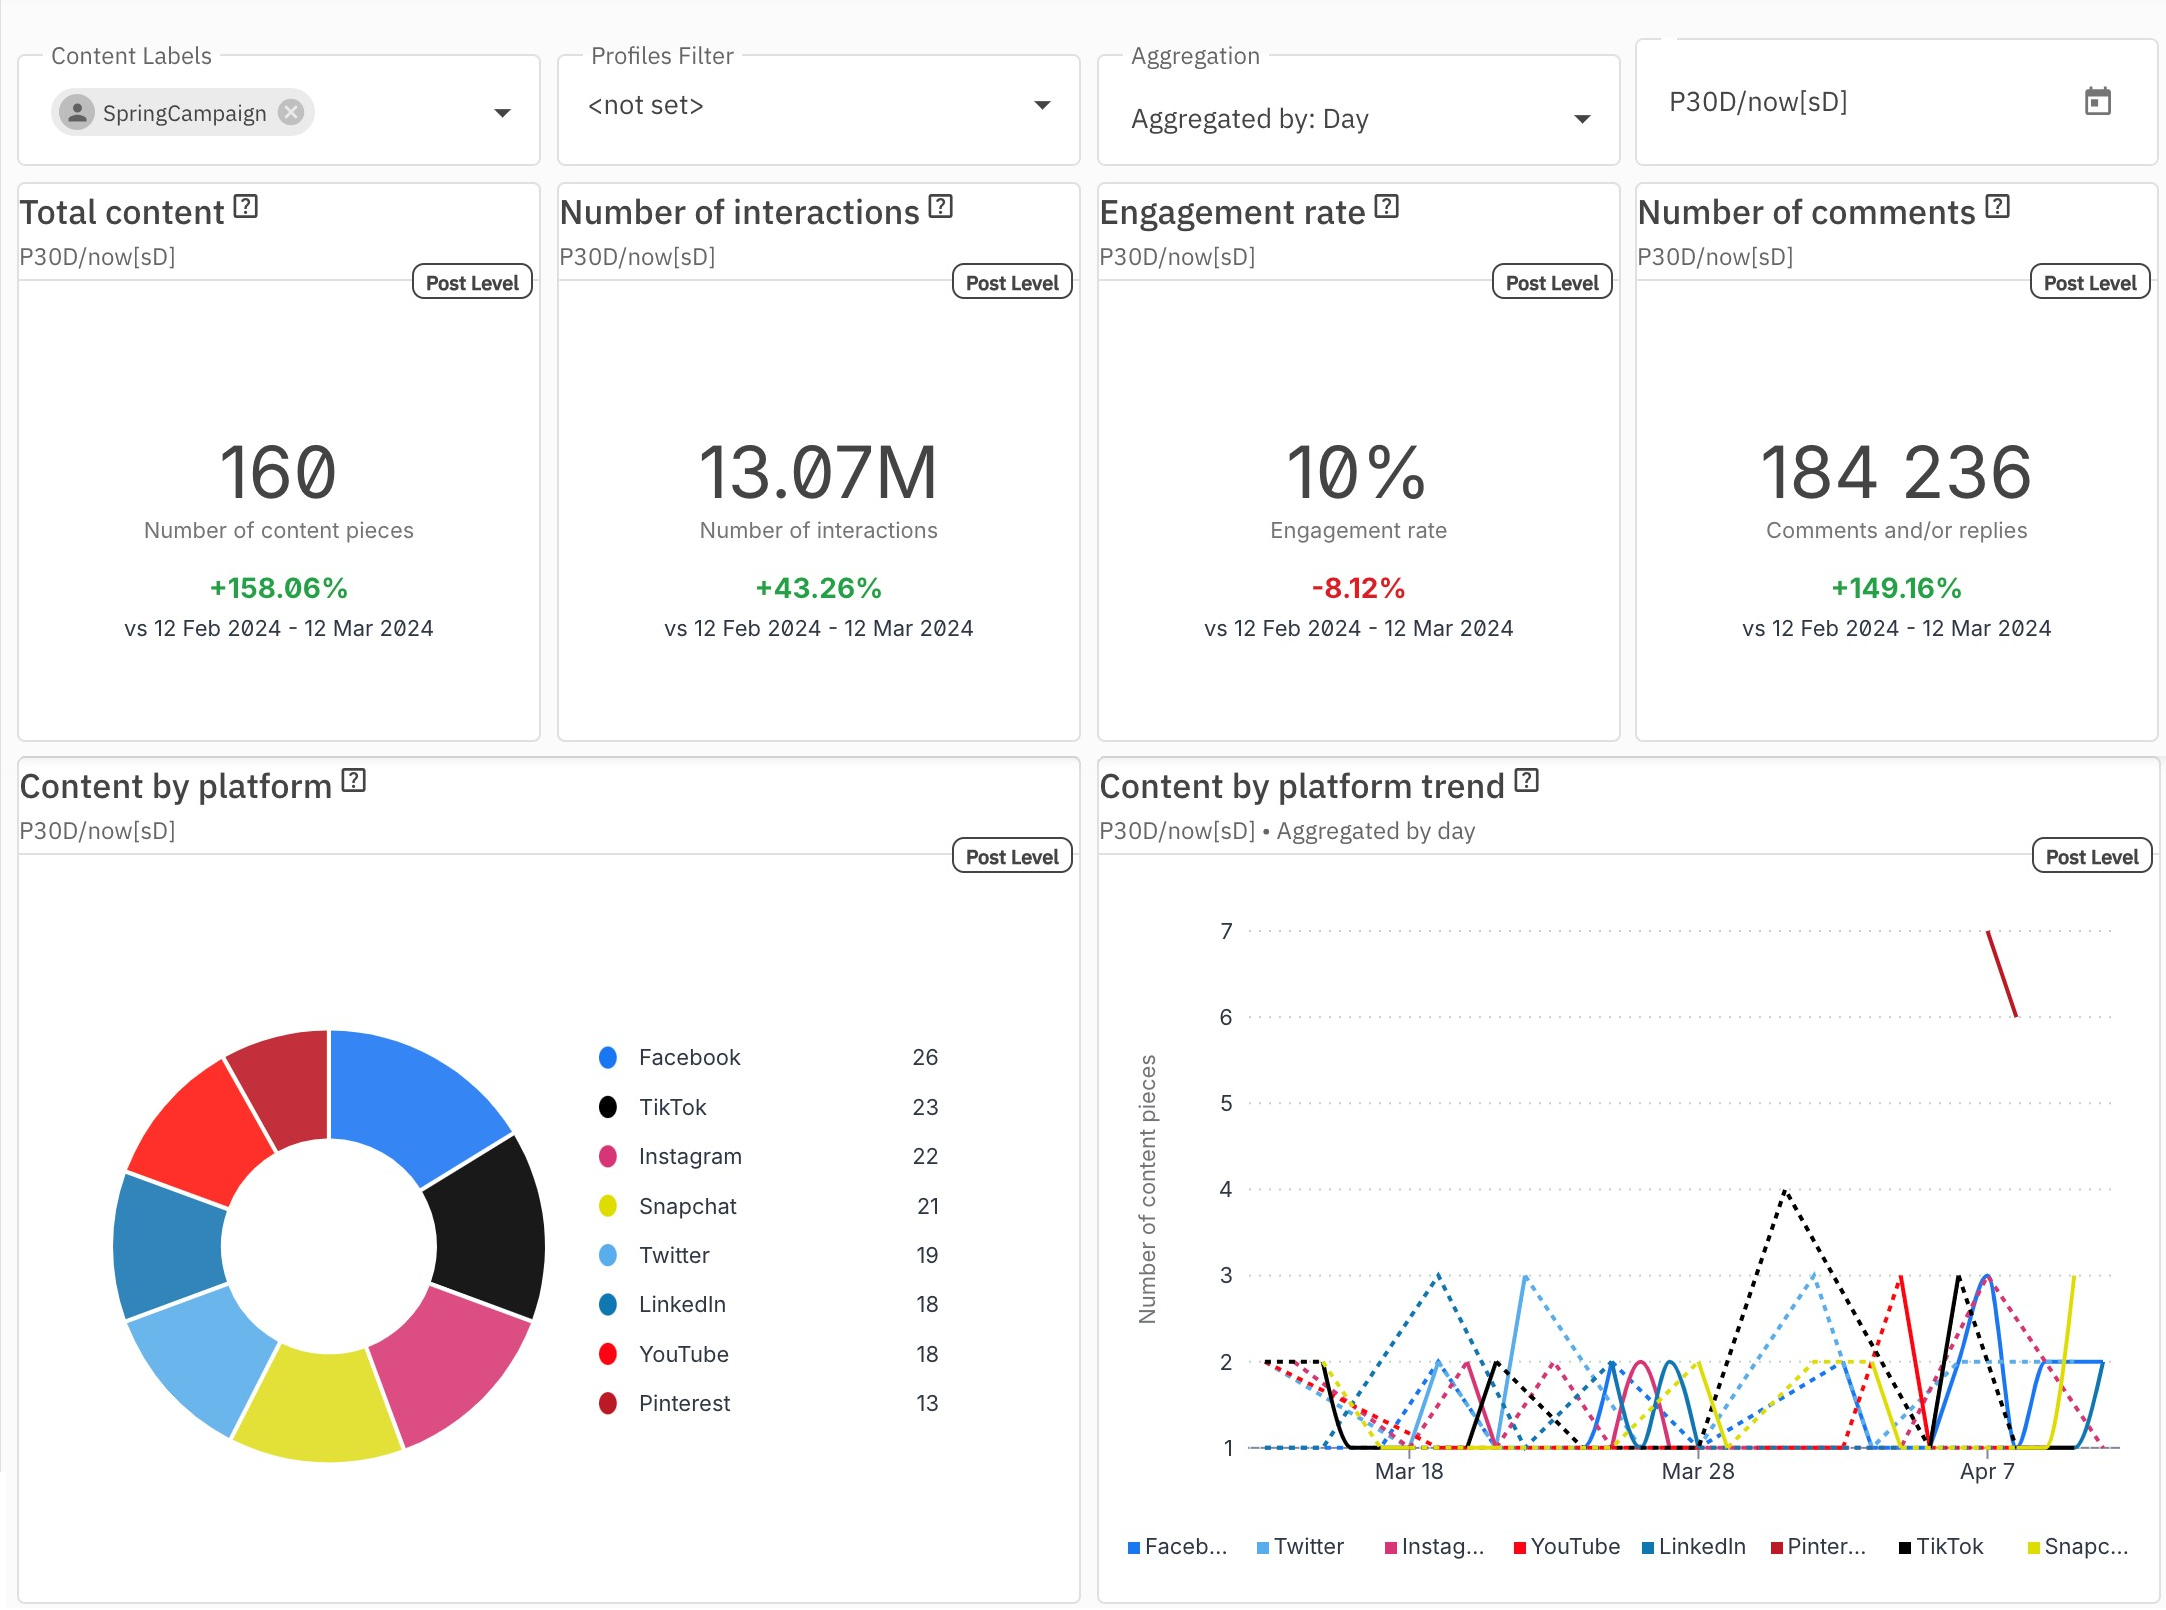
\includegraphics[width=1\textwidth]{pictures/omni-studio.png}
	\caption{Dashboard v Omni Studiu}
	\label{fig:omniStudioDashboard}
\end{figure}
Vidíme, že dasboard obsahuje nejen vizualizace, ale i ovládací prvky. Každý tento widget má svoje jedinečné ID, které je dostupné, pokud se rozklikne nastavení widgetu. Zároveň Omni Studio 
umožňuje uživateli zobrazit konfiguraci grafu (neexpandované), datové requesty (neexpandované) a i samotná data. V jedné ze sekcí widgetu jsou i tzv. debuggovací nástroje, ve kterých se nachází pole JSON parametrů,
které je dodefinovat, aby graf mohl být vykreslen. Na obrázku \ref{fig:omniStudioDashboard} je zřejmé, že uživatel pro realizaci vykreslení musel vybrat hodnoty v ovládacích prvkách (konkrétně 
časovou škálu, časovou agregaci a hodnotu labelu - hodnota pro filtry zůstala nevyplněná, jelikož je nepovinná - udává pouze omezení na datový request, pokud by chtěl uživatel data ještě nějak
dál extrahovat - např. filtrování na základě sociální sítě, typu interakcí apod.). 

Tyto hodnoty se následně převedou do pole JSON objektů a následně se při vizualizaci uplatní. Tím grafy zůstávají dynamické, protože při každé uživatelské interakci se ihned překreslí s novými
daty.

Tyto parametry budou klíčové pro správnou funkcionalitu knihovny - zajistí správné vykreslení a pokud nebudou v rámci aplikace specifikovány nějakými prvky (např. že by uživatelova aplikace obsahovala
inputy/výběrové seznamy pro všechny nespecifikované hodnoty), bude nutné je specifikovat ručně. To bude provedeno předáním přes properties React komponenty.

\subsection{Funkcionalita knihovny}
Knihovna tedy bude obsahovat obecnou komponentu \texttt{<Widget/>}, která bude reprezentovat právě jednu vizualizaci. Bude nutné komponentě předat číslo boardu, číslo widgetu a případně parametry, které 
budou expandovány knihovnou PreJSON v konfiguraci widgetu. Tato komponenta se postará o veškeré fetchování dat a následnou vizualizaci. Jelikož Vision knihovna vizualizuje pouze samotný graf, bude nutné, aby
Widget komopnenta uměla zobrazit i nadpisy, podnadpisy a další prvky obsažené v hlavičce. Bude tedy třeba zajistit základní stylování (např. fonty a velikost písma), ale uživateli bude umožněno vložení CSS stylů
opět přes propsu komponenty - to nabídne uživateli větší možnosti, jak si embedovaný graf sám vystylovat. Postup při vizualizaci bude vypadat přibližně takto:

\begin{enumerate}
	\item Uživatel zadá ID boardu a widgetu + další potřebné parametry
	\item Komponenta provede veškerá potřebná volání - stáhne konfigurace, proběhne expandace konfigů apod.
	\item Aplikují se předané CSS styly 
	\item Výsledné zobrazení grafu
\end{enumerate}

Výsledná knihovna bude přístupná přes npm (Node Package Manager), což zajistí její snadné stažení a použití. Instalace bude vyžadovat pouze nainstalovaného správce balíčků npm a použití budete
detailně vysvětleno v uživatelské dokumentaci.

\section{Návrh UI}

Při navrhování uživatelského rozhraní (UI) je třeba myslet na UX (User Experience). Výsledné rozhraní musí být přehledné, uživatelsky přívětivé a nezasekávat se. Pro lepší UX bude rozhraní 
obsahovat nejen sekci pro správu tokenů, ale také sekci pro náhled embedovaných grafů a následné generování zdrojového kódu pro tyto náhledy. Tím se zvýší použitelnost tohoto UI, jelikož 
věci potřebné k embedování sloučí do jednoho UI (tj. bude se jednat o jednostránkovou aplikaci). Ze strany zadavatele je důraz především na funkcionalitu a UX, nikoliv na estetiku. Proto toto bude zohledněno při navrhování.

\subsection{Vytváření tokenů}

K vytvoření tokenů bude sloužit patička stránky. V ní se budou nacházet dvě tlačítka - jedno pro vytvoření Public API tokenu, druhé pro Omni API token. K vytvoření těchto tokenů je třeba být přihlášen v
účtu Suite, jak bylo dřívě zmíněno. Po stisknutí tlačítka bude uživatel přesměrován na stránku, kde udělí patřičné oprávnění, že se pro jeho účet vytvoří token. Po potvrzení se uživateli token uloží
do local storage webového prohlížeče. To umožní okamžitou možnost embedování v UI a zároveň snadnou přístupnost k tomuto tokenu. Pokud bude chtít uživatel token používat ve své aplikaci, jednoduše jej z local storage
zkopíruje k sobě do aplikace, kde jej bude dále moci normálně využívat. To by platilo pro případ, kdy by jeden z tokenů vypršel. Ovšem bude-li uživatel nový a bude nutno vygenerovat oba dva tokeny pro potřebné vizualizace,
bude přidáno tlačítko, které uživateli zkopíruje oba dva tokeny ve formátu \texttt{.env} souboru. Uživatel tedy nebude muset sám hodnoty přepisovat, ale pouze je vloží zkopírované do \texttt{.env} souboru. Zkopírované tokeny
budou ve formátu:
\lstset{style=plainsrc}
\begin{lstlisting}
ACCESS_TOKEN=pis4185dfgfdesfDs5asd
OMNI_API_TOKEN=s5Z9sB=Fd--lK67a44ed12
\end{lstlisting}

\subsection{Náhled vizualizací}
Součástí uživatelského rozhraní bude také sekce pro náhled na vizualizované grafy. Ten bude obsahovat základní uživatelské vstupy (všechny, které bude přijímat výsledná komponenta z naimplementované knihovny), 
díky kterým se vizualizace budou moci rychle ovládat a vykreslovat. Pro rychlé embedování bude vytvořeno i tlačítko, které otevře uživateli dialog, v němž bude vygenerovaný zdrojový kód, kterým by se
v jeho aplikaci daný graf vykreslil. Výstup bude vypadat zhruba takto:

\lstset{style=plainsrc}
\begin{lstlisting}
<Widget widgetID={1598} boardID={12} 
params={{time:"now"}} width={500}/>
\end{lstlisting}


\section{Dokumentace}

Výstupem bude i podrobná dokumentace - a to jak uživatelská, která bude specifikovat použití pro koncové uživatele, tak i programátorská, která bude obsahovat souhrn informací potřebné
pro další vývoj. Dokumentace bude obsahovat následující body:

\begin{enumerate}
	\item Instalaci knihovny a její následnou integraci do uživatelovi aplikace
	\item Stručný návod k používání uživatelského rozhraní pro obnovu tokenů
	\item Sekci pro vývojáře
\end{enumerate}

Přístupu k dokumentaci je několik - od stručného souboru \texttt{.pdf} až po samostatnou webovou aplikaci. Aby dokumentace byla přehledná a snadno rozšiřitelná, bude dokumentace statická stránka
přístupná na veřejné URL adrese. Pro tuto možnost využijeme Docusaurus - generátor statických stránek určen pro generaci právě uživatelských dokumentací. 

Docusaurus umožní ze souborů s příponou .md (soubory běžně používané pro dokumentace v gitových repozitářích) zbuildit statickou webovou stránku, která uživateli poskytne přehledné 
rozhraní. Výsledná dokumentace bude vydána na veřejné internetové stránce, aby k ní byl snadný přístup odkudkoliv.


\chapter{Implementace}
Tato kapitola popisuje implementaci knihovny a uživatelského rozhraní. Jako první bude vyvíjena knihovna, protože následně bude rovnou využívána uživatelským rozhraním pro
náhled vizualizací.

\section{Implementace knihovny}

\subsection{Vývoj knihovny v čase}

Pro okamžité testování funkcionality byla knihovna nejprve vyvíjena formou React aplikace, která byla po implementaci všech potřebných funkcionalit převedena na knihovnu.
Zároveň v době vývoje nebyly ještě zadavatelem vystaveny endpointy na Omni Studio API v rámci Public API. Aplikace tedy pracovala přímo s Omni Studio API, z čehož ale vyplývá,
že pro vyvíjení bylo třeba být připojen na firemní VPN. To samé platilo i pro správné fungování - spustil-li uživatel aplikaci lokálně a nebyl připojen na VPN, grafy nemohly být vykresleny,
protože aplikace neměla přístup k Omni Studio API. 

Pro frontend aplikace byl použit framework React a další knihovny jako např. MUI, tanstack react query apod. Backendová část byla psána v Node.js. Backend používal webový server express - ten
řešil veškeré načítání a posílání dat. Kód byl členěn do dvou hlavních složek - \texttt{server} a \texttt{client}. Adresář \texttt{server} obsahoval inicializaci backendu a následné nastvení a spuštění webového serveru. Naopak
adresář \texttt{client} obsahoval funkcionální komponenty k vykreslování embedovaných grafů a pomocné funkce, které sloužily k přeposílání dat z frontendu na backend či opačně. Jakmile aplikace
dokázala vykreslovat libovolné grafy, byla transformována z React aplikace do samotné JavaScriptové knihovny.

\subsection{Struktura knihovny}

Výsledná transformovaná knihovna má následující strukturu:

\dirtree{%
    .0 {}.
    .1 \faFolder{} docs.
	.1 \faFolder{} scripts.
		.2 \faFile[regular]{} postinstall.sh.
    .1 \faFolder{} src.
        .2 \faFolder{} client.
        .2 \faFolder{} server.
        .2 \faFolder{} tests.
        .2 \faFile[regular]{} index.js.
        .2 \faFile[regular]{} backend.js.
    .1 \faFile[regular]{} .babelrc.
	.1 \faFile[regular]{} .gitignore.
    .1 \faFile[regular]{} .mocharc.json.
    .1 \faFile[regular]{} .npmignore.
	.1 \faFile[regular]{} .prettierrc.js.
    .1 \faFile[regular]{} README.md.
	.1 \faFile[regular]{} package-lock.json.
    .1 \faFile[regular]{} package.json.
    .1 \faFile[regular]{} webpack.config.js.
}

Veškeré složky či soubory uvedené ve výše zmiňovaném adresáři jsou podrobně popsány v tabulce \ref{tab:dirLibrary}


\begin{center}
	\begin{longtable}{p{.25\textwidth}p{.6\textwidth}}
	\caption{Obsah knihovny}
	\label{tab:dirLibrary}\\
	\toprule[1.5pt]
	\endhead
	\midrule
	\multicolumn{2}{r}{\textit{(tabulka pokračuje na další stránce)}}\\
	\endfoot
	\bottomrule[1.5pt]
	\endlastfoot
	%
	\verb"docs" & Obsahuje složku s uživatelskou dokumentací generovanou Docusaurem. \\
	\midrule
	\verb"scripts" & Složka se souborem sloužící k nainstalování minifikovaných verzí interních knihoven. \\
	\midrule
	\verb"src/client" & Složka s frontendovou implementací - veškeré React komponenty, konstanty a pomocné funkce určené k fetchování a zpracování dat.  \\
	\midrule
	\verb"src/server" & Složka s backendovou implementací - veškeré routy serveru Express určené k fetchování dat z API.  \\
	\midrule
	\verb"src/index.js" & Exportovaná frontendová část knihovny \\
	\midrule
	\verb"src/backend.js" & Exportovaná backendová část knihovny \\
	\midrule
	\verb".babelrc" & Slouží k definici přednastavené sady Babel pluginů, které se použijí k transformaci JavaScript kódu z jedné syntaxe do druhé.  \\
	\midrule
	\verb".mocharc.json" & Registruje mocha unit testy u babelu, aby mohly být spuštěny.  \\
	\midrule
	\verb".npmignore" & Specifije, které soubory budou při nahrávání na \url{https://www.npmjs.com/} ignorovány. \\
	\midrule
	\verb".prettierrc.js" & Soubor specifikující konfiguraci pro automatické formátování kódu. \\
	\midrule
	\verb"README.md" & Soubor pro uživatele pro rychlé porozumění projektu.  \\
	\midrule
	\verb"package-lock.json" & Soubor zajišťující konzistenci verzí závislostí v Node.js projektu a optimalizující proces instalace balíčků.  \\
	\midrule
	\verb"package.json" & Soubor obsahující metadata, závislosti a skripty pro projekt v Node.js. \\
	\midrule
	\verb"webpack.config.js" & Definuje, jak bude zdrojový kód knihovny zbuilděn.  \\
	\end{longtable}
\end{center}

\subsection{Postinstall skript}

Jelikož interní knihovny nebyly veřejné, bylo třeba je nějakým způsobem poskytnout. Nejprve připadala v úvahu možnost, že by se stahovaly pomocí npm, ovšem
nakonec se přistoupilo k možnosti, že knihovny budou stahovány pomocí Emplifi Public API. K jejímu stažení se bude uživatel muset prokázat platným přístupovým tokenem.
To zajišťuje i částečnou ochranu před neoprávněným stažením.

Stažení a následné uložení řeší bash skriptový kód v souboru \texttt{postinstall.sh}. Ten nejprve vytvoří složku \texttt{dist} a následně zkontroluje, zda je v systémové proměnné
nastavená hodnota tokenu a URL (\texttt{PACKAGE\_URL}), odkud knihovny stáhnout. Pokud hodnoty nastavené nejsou, automaticky bude brát hodnoty z \texttt{.env} souboru. Následně pomocí CURL pošle dotaz na
specifikovanou URL, v těle přiloží přístupový token a výsledek uloží do souboru \texttt{embedding.js} ve složce \texttt{dist}.

Tento skript se automaticky spouští při instalaci dependencí této knihovny - je tedy před samotnou instalací zajistit, aby byl zajištěn přístup k platnému tokenu a URL adrese.

\subsection{Backendové routy}

Jak již bylo zmíněno, výstupem knihovny budou mimo jiné i routy serveru Express, které budou zajišťovat a zprostředkovávat komunikace s API.

Výstupem jsou tři backendové routy, které slouží ke stažení widget konfigurace, kte stažení dat pro widget a ke stažení dashboard fieldů (jejich význam bude vysvětlen u samotného vykreslování).
Routy pro widget konfigurace a dashboard fieldy jsou typu GET - ten slouží zejména ke čtení dat, nikoliv upravování, mazání či vkládání. Obě tyto routy přijímají v parametru requestu ID
dashboardu a následně provedou volání na API. 

Token je možné specifikovat dvěma způsoby - a to buď specifikováním v \texttt{.env} souboru či systémové proměnné, nebo předání v hlavičce requestu. To umožňuje větší použitelnost pro koncového
uživatele - jak bude zmíněno např. v implementaci uživatelského rozhraní. Routy následně vrací data na frontend ve formátu JSON. Došlo-li při fetchování dat k chybě, je vrácena chyba.

Třetí routa je typu POST - POST zpravidla slouží k získání dat, ale oproti metodě GET obsahuje i tělo, kterým může předávat potřebné parametry či specifikace. To samozřejmě může být provedeno i
použitím GET, ale v praxi se toto užití nedoporučuje kvůli tomu, že hlavička requestu GET by byla pak velmi dlouhá. V tomto případě předáváme v tělu POST requestu cestu k endpointu, ze kterého data
fetchovat, a dále payload. Payload je objekt, který definuje dotaz na data - specifikuje jak data filtrovat, agregovat, řadit apod. 

Všechny tři routy využívají k fetchování dat z Public API knihovnu axios. Následně jsou tyto routy vyexportovány jako jeden Express router, aby bylo možné jejich další použití v jiných částí projektu.

\subsection{Organizace frontendové části}

Frontendová část obsahuje kromě konstant, komponent a funkcí i soubor \texttt{.eslintrc.js}. Tento soubor slouží jako konfigurace pro plugin ESLint, který slouží ke statické analýze
kódu - upozorňuje a pomáhá odstraňovat nekonzistence či špatné praktiky v kódu. Díky tomuto pluginu kód neobsahuje např. zbytečné importy a deklarace komponent, které se v kódu nijak nevyskytují,
upozorňuje na chybějící dependence u React hooků či validuje předané properties.

\subsubsection{Adresář constants}

Adresář obsahuje dva soubory. První soubor \texttt{api-messages.js} obsahuje konstanty pro chybové výpisy (při fetchování dat z API, nevalidních PreJSON parametrech apod.).
Druhý soubor \texttt{prejson-type.js} obsahuje mapu pro knihovnu PreJSON. PreJSON knihovna se naimportuje z minifikovaného souboru a následně se vytvoří mapa, která specifikuje
pro hodnoty widgetů jejich PreJSON typ. Ta je poté využívána při deklaraci datového typu dashboard fieldu (zmíněno v nadcházející kapitole).

\subsubsection{Adresář functions}

V tomto adresáři se nachází veškeré funkce, které se využívají k dotazování dat z frontendu na backend či funkce pro PreJSON.

Soubor \texttt{functions.js} obsahuje funkci určenou pro parsování řetězce na string. Byla vytvořena z důvodu jednoduché manipulace s uživatelovým vstupem. Není tedy třeba
testovat, zda je řetězec validní JSON objekt nebo ne, tato funkce vrátí buď zparsovaný JSON objekt, nebo hodnotu null.

Jelikož časový rozsah widgetů lze určit i řetězcem (např. hodnota P60D/now[sD] specifikuje posledních 60 dní), je třeba jej umět převést z tohoto řetězce. O to se stará soubor
\texttt{prejson-suite.js}, jehož výstupem je objekt, který tento časový úsek reprezentuje.

Veškeré funkce, které zpostředkovávají komunikaci mezi frontendem a backendovými routami, jsou specifikovány v souboru \texttt{widget-config.js}. Obsahuje 4 procedury pro výše zmiňované
volání - pro získání widget konfigurace, dat a dashboard fieldů. Widget může obsahovat více requestů na data (např. počet komentářů a počet celkových interakcí). Proto je nutné detekovat,
jak přistupovat k volání dat - je-li datový request objekt, zavolá se API jednou a výslednou návratovou hodnotou je opět objekt se staženými daty. Jestliže je ale datový request pole, jedná se o pole objektů, které specifikují request - je tedy
nutné iterovat postupně přes všechny requesty v poli pomocí funkce \texttt{map()}. Návratovou hodnotou bude v tomto případě pole dat.

\subsubsection{Adresář components}

Složka obsahuje veškeré React komponenty této knihovny. Hlavní komponenta, definovaná v souboru \texttt{widget.jsx}, slouží k vykreslení celého widgetu z Omni Studia. Jejím úkolem
je zpracování parametrů pro widget, stažení a načtení dat a následně jsou tyto hodnoty předány dceřinné komponentě pro vykreslení.

K funkcionalitě je nutno specifikovat několik parametrů, které jsou specifikované v tabulce \ref{tab:widgetProps}.

\begin{center}
	\begin{longtable}{p{.2\textwidth}p{.65\textwidth}}
	\caption{Properties komponenty <Widget/>}
	\label{tab:widgetProps}\\
	\toprule[1.5pt]
	\endhead
	\midrule
	\multicolumn{2}{r}{\textit{(tabulka pokračuje na další stránce)}}\\
	\endfoot
	\bottomrule[1.5pt]
	\endlastfoot
	%
	\verb"boardID" & Identifikátor dashboardu.  \\
	\midrule
	\verb"widgetID" & Identifikátor widgetu\footnote{Jedinými vyžadovanými parametry jsou \texttt{boardID} spolu s \texttt{widgetID}. Zbytek parametrů je nepovinný, je ale velice pravděpodobné, že může být potřebný ke správnému vykreslení (např. parametr \texttt{params}).}. \\
	\midrule
	\verb"params" & Pole parametrů potřebné k vizualizaci grafu \footnote{Tyto parametry jsou k nalezení v aplikaci Omni Studio. Detailní postup je zmíněn v uživatelské dokumentaci.}. \\
	\midrule
	\verb"className" & Jméno MUI třídy - specifikace stylu dle již existujících tříd. \\
	\midrule
	\verb"style" & Vlastní specifikace CSS stylu pomocí MUI komponenty \texttt{<Box/>}. \\
	\midrule
	\verb"width" & Šířka výsledné vizualizace (v pixelech). \\
	\midrule
	\verb"height" & Výška výsledné vizualizace (v pixelech). \\
	\midrule
	\verb"tokenFunc" & Funkce vracející tokeny, které jsou následně používány na backendu místo systémové proměnné. \\
	\end{longtable}
\end{center}

Nejprve se z pole parametrů vytvoří objekt. Tento objekt obsahuje vždy jméno atributu (což je název proměnné z Omni Studia, kterou je třeba dodefinovat) a k němu patřičná hodnota (specifikovaná
hodnota pro nedefinovaný parametr). Pokud se nejdná o pole, vrátí se prázdný objekt.

Následuje první stahování dat. Dle boardID předaného v properties se pošle request na API, který stáhne fieldy z daného boardu. Fieldy slouží k přesné specifikaci datového typu - např.
obsahuje-li konfigurace widgetu parametr \texttt{time}, specifikace hodnoty vypadat takto:
\lstset{style=plainsrc}
\begin{lstlisting}
...
key: "${time}"
...
\end{lstlisting}

Po obdržení fieldů z API je nutné tyto konfigurační předpisy rozšířit pomocí instance \texttt{PreJSONContext}. Po rozšíření vypadá specifikovaná hodnota takto:
\lstset{style=plainsrc}
\begin{lstlisting}
...
key: "${daterange:time}"
...
\end{lstlisting}

Dále je možno načíst konfiguraci widgetu, která obsahuje jak specifikaci vizualizace (barvy, popisky os, ...), tak i datové requesty. Opět se specifikuje číslo dashboardu, API stáhne veškeré widgety z toho boardu a následně se dle widgetID vyfiltrují na jeden vyhovující. Jestliže
neexistuje widget s daným ID, je vrácena chybová hláška o nenalezení widgetu a stahování dat neproběhne. Pokud byly specifikované identifikátory správné, dalším krokem je expandování
widget konfigurace. 

Pro expandaci je nejprve nutné převést datové requesty widget konfigurace do PreJSON objektu. Po úspěšné převedení dat se vezme námi vytvořený objekt s datovými requesty a vytvořenou instancí \texttt{PreJSONContext} se zkontroluje, zda-li uživatel zadal všechny parametry, které jsou
potřebné k expandování a následné vizualizaci. Pokud uživatel nezadal všechny ptořebné parametry, expandace neproběhne a uživatele o tom informuje chybová hláška. Pokud ale zadal 
všechny potřebné parametry, expanduje PreJSON objekt danými parametry a následně zkonvertuje do objektu JSON.

Posledním krokem je stažení dat. To proběhne pouze v případě, jestliže expandování datových requestů proběhlo v pořádku. Requesty jsou pak jeden po druhém postupně volány a vrácená data
uložena jako objekt/pole (jak bylo zmiňováno, pro více než 1 request bude návratový typ dat pole). Widget může obsahovat ale i hodnoty navrácených dat např. v nadpise či nápovědě.
To ovšem knihovna Vision neřeší, jelikož vykresluje pouze samotné vizualizace bez hlaviček. Proto je nutné ještě expandovat konfiguraci widgetu samotnými daty, kdyby se v hlavičce vyskytovala
hodnota závislá na datech (např. právě zmiňovaný počet datových reqestů). 

Proběhlo-li veškeré fetchování dat v pořádku, data, widget konfigurace a datové requesty jsou předány dceřinné komponentě k vykreslení. Jestliže nastala při načítání, zpracovávání či expandování dat
chyba, je vypsána místo samotné vizualizace. 

Než se výše popsané kroky provedou, bude třeba indikovat načítání komponenty - zejména pokud datových requestů bude více a bude nutné posílat více dotazů na API. Tento stav bude velmi jednoduché 
detekovat, protože používaná fetchovací funkce \texttt{useQuery()} vrací nejen načtená data, ale také dokáže indikovat, zda-li došlo při stahování k chybě nebo jestli stahování stále probíhá. Proto
je pro všechna tři načtení udržován stav \texttt{useQuery()} \texttt{isLoading} (pro každou funkci samozřejmě přejmenován na jiný název proměnné). Díky nim lze snadno vizualizovat, zda se vizualizace stále načítá.
Pro tuto indikaci je použita předdefinovaná komponenta \texttt{<CircularProgress/>} z knihovny MUI.

Výhodou používání \texttt{useQuery()} je také zmiňované cachování. Každé volání \texttt{useQuery()} má svůj klíč a jestliže již data byla jednou žádána s tímto klíčem,
nebude se provádět volání na backend a API, ale rovnou se načtou z cache. Díky tomu se widget vykreslí téměř okamžitě, protože již veškerá potřebná data k vizualizaci obsahuje. 

V neposlední řadě užívání \texttt{useQuery()} umožňuje aktivovat dané volání pouze za předpokladu, že jsou splněny specifikované podmínky. To zajišťuje atribut \texttt{enabled},
což je podmínka, která jestliže je splněna, tak se spustí stahování dat. Toto usnadnilo při implementaci práci zejména tím, že nebylo nutné si držet vlastní stavy a díky tomu
je kód čitelnější.

Nehledě na výsledek a stav vizualizace, uplatní se na výsledek této komponenty výška, šířka a styly předané přes properties. Pro budoucí rozšíření knihovny byla tato komponenta
naimplementována obecněji - tj. pokud proběhly veškeré data fetche v pořádku, ještě se zkontroluje, zda-li typ widgetu je opravdu "vision". Momentálně jiný typ widgetu ani podporován není,
ale komponenta je připravena v budoucnosti na podporu všech druhů widgetů.


Dceřinná komponenta \texttt{<WidgetVision/>} následně zpracovává přijatou konfiguraci a data a poté je vizualizuje. Nejprve zkontroluje hlavičku konfigurace (nadpisy, podnadpisy, tooltipy, ...),
předá data a widget konfiguraci komponentě \texttt{<Vision/>} a vykreslí patičku s informačním štítkem, že se jedná o data pocházející z Emplifi. Pro vývojářské a debuggovací účely jsou 
zřízeny i dvě komponenty. které vizualizují neexpandované a expandované datové requesty. Pokud uživatel nespecifikuje pomocí properties, že je chce vypsat, jsou automaticky ignorovány a nevykresleny.

\subsubsection{Sestavení knihovny}

Protože knihovna obsahuje frontendovou část i backendovou část, výstupem budou dva soubory. Pro přehlednost jsou exportované komponenty a routy v kořenu adresáře \texttt{src}. Zároveň používání
funkce \texttt{useQuery} vyžaduje tzv. QueryProvidera. Proto při exportu \texttt{<Widget/>} je komponenta vložená do komponenty \texttt{<QueryClientProvider/>}, která přijímá v properties instanci
Query Clienta. Tato komponenta obohacená o Query Clienta je poté vyexportována jako normální \texttt{<Widget/>} komponenta a uživatel tedy nemusí ve svém projektu tohoto Query Clienta vytvářet.

Pro sestavení knihovny se využívá modul webpack. Jeho konfigurace je uložená v kořenovým adresáři knihovny a obsahuje dvě konfigurace pro buildění - pro frontendovou část a backendovou.
Na sestavení knihovny je následně vytvořen skript, který je definovaný v \texttt{package.json} a spouští se pomocí npm. Výsledné dva vytvořené soubory (\texttt{empli-embed-backend.js} a \texttt{empli-embed.js})
jsou uloženy do složky \texttt{dist}. Poté už je třeba jen aktualizovanou verzi knihovny zveřejnit na \url{https://www.npmjs.com/}. Pro tuto akci je taktéž vytvořen skript v \texttt{package.json}.
Podrobnější informace jsou v uživatelské dokumentaci.

\section{Implementace uživatelského rozhraní}

\subsection{Importování knihovny}

Jelikož uživatelské rozhraní bude sloužit i k náhledům na vizualizace, je nutné knihovnu naimporovat (je ale nutné ji instalovat do již existujícího projektu). Protože se ale knihovna nachází na npm, bude to velice snadné.
Postup i průběh je znázorněn na výpisu: 
\setwinprompt{C:/Users/janochmi/ReactProjects/init_example}
\begin{console}{Instalace knihovny}
`\winprompt` npm i empli-embed

added 159 packages, and audited 160 packages in 19s

30 packages are looking for funding
  run `npm fund` for details

found 0 vulnerabilities
\end{console}

Knihovna se nainstalovala a dalším krokem je inicializace React aplikace, která bude tuto knihovnu používat.

\subsection{Inicializace aplikace}

Uživatelské rozhraní je jednostránková aplikace s frontendovou i backendovou částí. Nejprve bylo třeba nainicializovat backendovou část. Jelikož knihovna obsahuje routy pro webový
server Express, bylo nutné tyto routy přidat do námi vytvořeného routeru, který mimo jiné obsahuje i vlastní routy pro tvorbu tokenů (bude zmíněno v dalších kapitolách). To je předvedeno na
ukázce \ref{expressInit}.

\begin{lstlisting}[language=Javascript, caption={Inicializace Express serveru}, label=expressInit]
	const express = require('express')
	// Requiring library routes
	const { routes } = require('empli-embed') 
	// Other requirements ...
	const apiRouter = require('./api-router')
	const nonApiRouter = require('./non-api-router')
	// Other actions ...
	const app = express()
	app.use(express.json())
	app.use('/api', routes, apiRouter, nonApiRouter)
	// Other actions ...
	app.listen(...)
\end{lstlisting}

Po úspěšném nastavení serveru je možné přejít na inicializaci frontendu aplikace. Je opět nutné naimportovat knihovní komponenty jako na ukázce \ref{reactIniti}.
\begin{lstlisting}[language=Javascript, caption={Inicializace React komponenty}, label=reactIniti]
	import { Widget } from 'empli-embed'
	// other code ...

	export default const App = () => {
		return <Widget boardID={100} 
				widgetID={51989} params={...}/>
	}
\end{lstlisting}

Nyní je inicializace aplikace dokončena. 

\subsection{Vytváření tokenů}

Nejprve bylo nutné připravit grafické rozhraní pro patičku stránky. Ta obsahuje dvě tlačítka pro generaci tokenů a jedno pro kopírování těchto tokenů. Tyto tlačítka
jsou importována z knihovny MUI, jelikož obsahují již předdefinované styly a nabízí i více funkcionalit (např. vkládání ikon na začátek/konec tlačítka, definici velikosti
tlačítek přes argument apod.). Každé tlačítko má přiřazen label, který indikuje, o jaký token se jedná. Tento label je realizován pomocí MUI komponenty
\texttt{<Tooltip/>}, která při najetí kurzoru myši na daný label zobrazí i dodatečný titulek (v tomto případě indikuje stav tokenu - je-li platný, neplatný či jestli vypršel).


\subsubsection{Public API token}
K vytvoření Public API tokenu je nutné být přihlášen v produktu Suite. Uživateli je po stisku tlačítka otevřena v novém okně stránka produktu Suite, kde udělí patřičné souhlasy. 
Toto přesměrování je realizováno tak, že při každém stisku tlačítka je vygenerováno uživateli ID requestu. Toto ID se uloží na serverový backend jako objekt do pole s nainicializovanou
hodnotou tokenu \texttt{null}. Mezitím se frontend každých 500 ms dotazuje metodou aktivního čekání, zda se již pro jeho request vygeneroval token. To se ověřuje pomocí kontrolování hodnoty
tokenu v objektu - je-li objekt stále \texttt{null}, probíhá kontrola stále dokola, dokud token není vygenerován a nebo uživatel nezavře stránku uživatelského rozhraní.

Přesměrování na stránku suite probíhá způsobem, který byl popsán v návrhu aplikace. Z frontendu se aplikace provolá na backendovou routu, která následně přesměruje nové okno
na URL vygenerovanou funkcí \texttt{getPublicApiCallbackUrl()}. Tato funkce přidá do URL adresy OAuth providera potřebné parametry zmíněné v tabulce \ref{tab:allParametersAPI}.
Až uživatel udělí patřičná oprávnění, na URL specifikovanou v \texttt{redirect\_uri} je zaslán autorizační kód. Tento kód se zachytí na backendu aplikace a
vytvoří se nový dotaz pro API. Zde je nutné se autorizovat pomocí klientského ID a secretu. O to se stará funkce \texttt{getAuthorization()}, která je zmíněna na 
ukázce \ref{autorHeader}. Klientské ID a secret musí být uložené v systémové proměnné (nebo \texttt{.env} souboru), aby bylo možné autentizaci provést.

\begin{lstlisting}[language=Javascript, caption={Vytvoření autozirační hlavičky pro následnou autentizaci}, label=autorHeader]
function getAuthorization() {
	return `Basic ${Buffer.from(
		`${process.env.CLIENT_ID_PUBLIC_API}:
		${process.env.CLIENT_SECRET_PUBLIC_API}`
	).toString('base64')}`
}
\end{lstlisting}

Po přijetí odpovědi z API se v poli requestů vyhledá request s uživatelovým ID. Tato hodnota je vložena při dotazech do parametru \texttt{state}, a proto můžeme snadně
určit, pro které ID requestu (respektive uživatele) se token vrátil. Po nalezení položky v poli se změní hodnota tokenu na obdržený token z Public API a automaticky se
zavolá skript na zavření okna, v němž uživatel uděloval oprávnění.

Na frontendu se po chvíli (500 ms) detekuje, že hodnota tokenu uloženého na backendu aplikace se změnila. Struktura tokenu byla uvedena v tabulce \ref{tab:exampleRequestResponse}.
Zbývá identifikovat, co z přijatých parametrů bude vhodné uložit. Uložit bude nutné \texttt{access\_token} a kvůli budoucímu rozšíření i \texttt{refresh\_token}. Tyto
dva tokeny se uloží do local storage, jak je uvedeno na ukázce \ref{savingPublicToken}.

\begin{lstlisting}[language=Javascript, caption={Ukládání Public API tokenů do local storage}, label=savingPublicToken]
	localStorage.setItem('public-api-access-token', 
	token.access_token)
	localStorage.setItem('public-api-refresh-token', 
	token.refresh_token)
\end{lstlisting}

\subsubsection{Omni API token}
K vytvoření Omni API tokenu je nutné být přihlášen na firemní VPN. Princip je velmi podobný. Uživateli se otevře nové okno, kde je přesměrován na stránku Omni Studia, kde je požádán
o souhlas. Po potvrzení je opět na \texttt{redirect\_uri} zaslán autorizační kód. Nyní je třeba zaslat dotaz na Omni APi, které je ovšem schované za VPN. Zadavatel ovšem pro tento případ
vystavil zmiňovaný endpoint na Public API. Do těla requestu se uloží parametry pro Omni API (znázorněno na ukázce \ref{omniApiCall}) a následně se provede volání na vystavený endpoint
\texttt{/3/omni-studio/oauth2/token}. 

\begin{lstlisting}[language=Javascript, caption={Parametry pro Omni API}, label=omniApiCall]
body: JSON.stringify({
		headers: {
			Accept: 'application/json',
			'Content-Type': 'application/x-www-form-urlencoded',
			Authorization: `Basic ${Buffer.from(
				`${process.env.CLIENT_ID_OMNI_STUDIO}:
				${process.env.CLIENT_SECRET_OMNI_STUDIO}`
			).toString('base64')}`,
		},
		body: `grant_type=authorization_code&
		code=${res.req.query.code}&redirect_uri=${uri}`,
}),
\end{lstlisting}

Jak je vidět, i pro Omni API je třeba autentizace formou klientského ID a secretu, ale jak je vidět, jedná se o jiné hodnoty než v Public API. Pro každé API
je tedy třeba jiného ID a secretu. Po vrácení tokenu z API je opět v poli requestů nalezen objekt s daným request ID, hodnota tokenu v objektu je nahrazena přijatou hodnotou a okno, v němž
uživatel uděloval oprávnění, je zavřeno. 

Pole pro requesty jsou dvě - jedno pro Public API, druhé pro Omni API. Nevýhodou při fetchování Omni API tokenu je ta, že v systémové proměnné musí být platný token - uživatel nemá jak předat
backendové routě, která zachytává kód vrácený z API, svůj Public API token (pokud je vůbec vygenerován). Proto je třeba, aby toto rozhraní v systémové proměnné (prozatím) obsahovalo stále platný 
Public API token. Výhodou ale je, že uživatel není omezen tím, jaký token vygeneruje první.

Opět se na frontendu metodou aktivního čekání každých 500 ms kontroluje, zda-li se token objevil v poli requestů na backendu a následně se ukládá do local storage jako na ukázce
\ref{savingOmniToken}.

\begin{lstlisting}[language=Javascript, caption={Ukládání Omni API tokenů do local storage}, label=savingOmniToken]
	localStorage.setItem('omni-studio-api-access-token',
	 token.access_token)
	localStorage.setItem('omni-studio-api-refresh-token',
	 token.refresh_token)
\end{lstlisting}
	
\subsubsection{Kontrola validity tokenů}

Při otevření stránky či po každém nastavení nového tokenu se spustí automaticky funkce \texttt{checkTokenAvailability()}, která kontroluje platnost tokenů. Pokud se v local storage nenachází
žádná hodnota pro token, je automaticky token nastaven na nevalidní a nastavena informační hláška při najetí myší na daný label tokeun. Pokud se ovšem nachází v local storage nachází
nějaká hodnota (ať už platný token, tak i ten nevalidní), vezme se daná hodnota a pošle se jako autorizační token v dotazu na API. Pokud API vrátí validní data, je zřejmé, že token je platný.
Na frontendu se následně nastaví validita tokenu na \texttt{true} a zlačítko pro obnovení tokenu zmizí a je nahrazeno zelenou checkmark ikonkou. Pokud ale API vrátí chybovou hlášku, 
vezme se tato chybová hláška a uloží se do informační hlášky labelu, token bude stále nevalidní a tlačítko se bude stále zobrazovat. 

\subsubsection{Zkopírování tokenů}

Pro tuto funkcionalitu je vystaveno tlačítko, které po stisknutí uloží do clipboardu oba dva tokeny (jak Omni API, tak Public API) a umožní je tak ihned
manuálně vložit do \texttt{.env} souboru. K tokenům je možné stále přistupovat i přes local storage, ale tato varianta je méně uživatelsky přívětivější než jedno stisknutí tlačítka.



\subsection{Náhled vizualizací}
% tady pak hlavně zmínit ten redux - ten to také dost natáhne - a jednotlivé modaly
Pro zobrazování náhledů vizualizací je třeba mít v local storage platné tokeny. Pokud platné nebudou, aplikace automaticky nastaví parametr tlačítko
\texttt{disabled} na \texttt{true}. Pro veškeré parametry, které přijímá komponenta \texttt{<Widget/>}, jsou vytvořeny vlastní ovládací prvky.
Pro boolean hodnoty jsou to přepínače, pro JSON objekty (parametry a CSS styly) a číselné hodnoty jsou to textová pole. Všechny tyto komponenty
jsou importovány z knihovny MUI.

Hodnoty těchto parametrů jsou ukládány v Redux storu. Tento reduxový store obsahuje dva reducery: 

\begin{enumerate}
	\item playground - spravuje hodnoty \texttt{<Widget/>} parametrů 
	\item playgroundUI - spravuje stavy dialogů (které z dialogových oken je otevřené)
\end{enumerate}

V playgroundu (vzniklý název pro toto výsledné UI) je nutné umět k těmto hodnotám přistupovat a měnit je. K tomu slouží funkce \texttt{useSelector()} a \texttt{useDispatch()},
které je třeba naimportovat. Pro přístup ke stavu je využita funkce \texttt{useSelector()}, která vrací objekt s destruktorovanými proměnnými z Redux storu. Naopak funkce 
\texttt{useDispatch()} slouží k odesílání akcí do Redux storu, které které umožňují měnit stav aplikace. Dále je třeba naimporovat z jednotlivých sliců action creatory, které
slouží k vytvoření příslušné akce, jež může následně upravovat stav aplikace. Změna aplikačního stavu je pak prováděna např. následujícím příkazem:

\begin{lstlisting}[language=Javascript]
onChange={() => dispatch(changeBoardID(event.target.value))}
\end{lstlisting}

V této ukázce reaguje komponenta na změnu hodnoty v poli. To spustí anonymní funkci, která volá \texttt{dispatch()} a předává ji výsledek volání \texttt{changeBoardID()}. Kromě parametrů
importujeme ze storu i proměnné pro stav tokenů, stav vizualizace či validitu JSON parametrů. Veškeré hodnoty jsou automaticky inicializovány na hodnotu \texttt{null} nebo \texttt{false}.

Při stisku tlačítka pro náhled se nejprve ověří, jsou-li vyplněné parametry čísla widgetu a boardu. Následně se do URL parametrů nastaví hodnoty všech proměnných z Redux storu
používané pro \texttt{<Widget/>} komponentu. Pro změnu stavu je \texttt{dispatch()} funkcí změněn stav vizualizace a začne se vykreslovat náhled vizualizace (ten reaguje automaticky
na změnu stavu vizualizace). Pro playground jsou tedy nutné dva stavy - jeden indikující hodnoty v uživatelských prvcích, druhý pro správu vizualizace (pokud by se používal pouze jeden,
znamenalo by to, že při každé změně hodnoty by se graf začal automaticky překreslovat, což by bylo velmi nepraktické).

Po úspěšném vykreslení vizualizace je zobrazeno tlačítko pro embedování. To otevře dialog, v němž uživatel vidí vizualizovaný graf a zdrojový kód, kterým je tento graf možné vykreslit.
Tento kód lze snadno zkopírovat do clipboardu a vložit do již existující aplikace, kde se následně vykreslí. Do výsledného zdrojového kódu se přidávají jen specifikované parametry -
prochází se veškeré parametry a filtrují se ty, jejichž hodnota je \texttt{null}. Ty, které zbyly, budou obsaženy ve výsledném zdrojovém kódu. Výsledný zdrojový kód nebude tedy vypadat následovně:
\begin{lstlisting}
	<Widget boardID={108} widgetID={187} height={null}
	width={null} params={{time:"now"}} style={null}/>
\end{lstlisting}
ale pouze takto:
\begin{lstlisting}
	<Widget boardID={108} widgetID={187} 
	params={{time:"now"}}/>
\end{lstlisting}

\subsection{Dokumentace}

Při implementaci knihovny byly vytvářeny Markdown (\texttt{.md}) soubory, které popisují důležité části knihovny a aplikace. Následně nástroj Docusaurus tyto soubory zkompiloval,
aby vytvořil webovou stránku, která je přístupná pro uživatele. Tímto způsobem byla vytvořena přehledná dokumentace, která slouží jako důležitý zdroj informací nejen pro koncové uživatele,
ale také pro vývojáře. Zdrojové soubory výsledné dokumentace se nachází ve složce \texttt{docs} uložené ve zdrojovém kódu knihovny. Návod na její použití se nachází v příloze \ref{app:docuDocs}.

\chapter{Testování}
Při testování byl kladen velký důraz na správnou funkcionalitu a stabilitu knihovny. Výsledná knihovna byla testována jednotkovými testy a testováním podle
scénářů. Jednotkové testy pokrývají 100\% výkonného kódu (testováno nástrojem istanbul/nyc, který zkoumá míru pokrytí kódu testy), což zahrnuje testování všech funkcí a komponent, 
které jsou přímou součástí implementace knihovny.
Tyto testy ověřují správnost a spolehlivost výkonného kódu v různých scénářích a podmínkách.

Pro provedení těchto jednotkových testů byl využíván testovací framework Mocha, který poskytl robustní a flexibilní prostředí pro psaní a spouštění testů. 
Díky Mocha bylo možné snadno definovat a organizovat testovací scénáře a sledovat jejich výsledky.

Je však důležité poznamenat, že některé části funkcionality, jako například mapování datových typů z PreJSONu, jsou pevně definovány a standardizovány v rámci specifikace knihovny nebo externích závislostí. 
Z tohoto důvodu není nutné testovat tato mapování v rámci unit testů, protože jsou považovány za externě ověřené a stabilní.

Namísto toho se zaměřujeme na testování klíčových aspektů funkcionality, které mohou být náchylnější k chybám a které mohou ovlivnit výkon nebo spolehlivost knihovny. 
Tímto přístupem zajišťujeme, že naše unit testy jsou účinné a efektivní ve zjišťování a prevenci chyb v implementaci naší knihovny.

Pro jednotkové testy bylo také nutné využít mockování. Veškerá mockovaná data jsou uložena v samostatném souboru a jsou předávána při volání API, 
což zajišťuje konzistentní a opakovatelné prostředí pro testování.

Dále byla knihovna testována v rámci testování uživatelského rozhraní - opět probíhalo testování podle scénářů a testerem přímo ze zadavatelské firmy.

Během testování uživatelského rozhraní byla ověřována především uživatelská přívětivost, intuitivnost a funkčnost knihovny z pohledu reálných uživatelů. 
Tester ze zadavatelské firmy se podílel na identifikaci potenciálních problémů a nedostatků v uživatelském rozhraní a poskytoval cennou zpětnou vazbu ohledně použitelnosti a uživatelského zážitku.
Tímto způsobem jsme se snažili zajistit, že knihovna nejen splňuje požadavky a očekávání našich uživatelů, ale také poskytuje optimální uživatelský zážitek při interakci s aplikací.

Výsledkem tohoto testování bylo zdokonalení uživatelského rozhraní a identifikace potřebných úprav a vylepšení, které byly následně doimplementovány. Veškeré testovací scénáře
jsou uvedené v příloze \ref{app:testCases}.



%
%
%        CHAPTER Závěr
%
% _____________________________________________________________________________
%
\chapter{Závěr}
Cílem bakalářské práce bylo vytvoření JavaScript knihovny, která umožní uživatelům embedovat grafy do aplikací třetích stran skrze
Emplifi Public API. Důležitou součástí bylo i navržení uživatelského rozhraní pro vytváření přístupových tokenů.

Nejprve byly zmíněny možnosti embedování a již existující řešení včetně srovnání zpětných vazeb zákazníků. Velká pozornost byla také
věnována k srovnávání jednotlivých přístupů k API.

Při implementaci knihovny bylo klíčové nejen zajistit její funkčnost, ale také udržovat přehledný a efektivní kód.
Velký důraz byl kladen na správnou implementaci funkčních požadavků a na použití moderních technologií. 
Tímto způsobem byl kladen důraz na vytvoření knihovny, která je nejen spolehlivá a efektivní, ale také snadno rozšiřitelná a udržovatelná v dlouhodobém horizontu.

Při tvorbě uživatelského rozhraní byla věnována pozornost na dvě klíčové oblasti - bezpečnost a uživatelskou přívětivost. Při generování přístupových tokenů bylo dbáno na
bezpečnostní normy a osvědčené postupy, aby bylo zajištěno, že přístup k citlivým datům je řádně zabezpečen. 
Zároveň byl kladen důraz na uživatelskou přívětivost s cílem zajistit, že výsledné rozhraní je intuitivní a funkční.

Výsledkem práce je uživatelské rozhraní pro vytváření tokenů, veřejná knihovna, která umožňuje integrování vizualizací z interní aplikace Omni Studio
do aplikací třetích stran, a podrobná uživatelská dokumentace, která popisuje použití knihovny a rozhraní koncovým uživatelem.

Testování prokázalo, že knihovna i uživatelské rozhraní jsou stabilní, spolehlivé, schopné reagovat na nevalidní stavy a poskytovat uživatelům očekávanou funkcionalitu. 



\appendix
\chapter{Uživatelská dokumentace}\label{app:docuDocs}
Uživatelská dokumentace se nachází ve zdrojovém kódu ve složce \texttt{docs}. K jejímu lokálnímu spuštění je potřeba mít nainstalovaný npm.
Celý postup na lokální spuštění dokumentace je znázorněn na ukázce:

\setwinprompt{C:/Users/janochmi/ReactProjects/library/docs}
\begin{console}{Spuštění uživatelské dokumentace}
`\winprompt` npm i
`\winprompt` npm start

> docs@0.0.0 start
> docusaurus start

[INFO] Starting the development server...
[SUCCESS] Docusaurus website is running at: http://localhost:3000/

 Compiled successfully in 6.50s

client (webpack 5.90.3) compiled successfully
\end{console}

V konzoli se ukáže adresa, na které je dokumentace spuštěna. Pro účel bakalářské práce byla tato dokumentace
zveřejněna na adrese \url{https://embedding-docs.vercel.app/}. 

Dokumentace obsahuje i odkaz na GitHub repozitář se zdrojovým kódem. V něm se nachází i tato dokumentace vyexportovaná do souboru \texttt{.pdf} v adresáři \texttt{docs}. 

V tabulce \ref{tab:docsTabs} jsou popsány jednotlivé sekce, které dokumentace obsahuje.

\begin{center}
	\begin{longtable}{p{.25\textwidth}p{.6\textwidth}}
	\caption{Struktura uživatelské dokumentace.}
	\label{tab:docsTabs}\\
	\toprule[1.5pt]
	\endhead
	\midrule
	\multicolumn{2}{r}{\textit{(tabulka pokračuje na další stránce)}}\\
	\endfoot
	\bottomrule[1.5pt]
	\endlastfoot
	%
	\verb"Introduction" & Úvod do knihovny. \\
	\midrule
	\verb"Getting-started" & Obsahuje detailní postup instalace knihovny, nainicializování projektu a použití knihovny. \\
	\midrule
	\verb"Development" & Určeno pro budoucí vývoj. Popisuje strukturu knihovny či návody ke stažení,vývoji a publikování.\\
	\midrule
	\verb"Embedding-Studio" & Popisuje funkcionalitu rozhraní a návod k jeho použití. \\
	\end{longtable}
\end{center}

\chapter{Testovací scénáře}\label{app:testCases}
\section{Testování knihovny}
\subsection{Pozitivní scénáře}
Pro veškeré pozitivní scénáře budeme předpokládat správně nainicializovanou aplikaci s platnými tokeny.
\subsubsection{Vykreslení widgetu}
\begin{enumerate}
	\item Do \texttt{<Widget/>} komponenty zadáme číslo dashboardu a widgetu.
	\item Do atributu \texttt{params} vložíme potřebné parametry.
	\item Zobrazíme.
\end{enumerate}
Očekávaný výsledek je vykreslení vizualizace.

\subsubsection{Vykreslení widgetu s hlavičkou}
\begin{enumerate}
	\item Do \texttt{<Widget/>} komponenty zadáme číslo dashboardu a widgetu, který obsahuje v hlavičce prvky (nadpis, podnadpis, nápovědu apod.).
	\item Do atributu \texttt{params} vložíme potřebné parametry.
	\item Zobrazíme.
\end{enumerate}
Očekávaný výsledek je vykreslení vizualizace, která bude obsahovat veškeré prvky z hlavičky.

\subsubsection{Vykreslení widgetu s MUI styly}
\begin{enumerate}
	\item Do \texttt{<Widget/>} komponenty zadáme číslo dashboardu a widgetu.
	\item Do atributu \texttt{params} vložíme potřebné parametry.
	\item Do atributu \texttt{style} vložíme libovolný objekt s MUI styly.
	\item Zobrazíme
\end{enumerate}
Očekávaný výsledek je vykreslení vizualizace s aplikovanými MUI styly.

\subsubsection{Vykreslení widgetu s danou výškou/šířkou}
\begin{enumerate}
	\item Do \texttt{<Widget/>} komponenty zadáme číslo dashboardu a widgetu.
	\item Do atributu \texttt{params} vložíme potřebné parametry.
	\item Do atributů \texttt{width} a \texttt{height} vložíme námi zvolené číselné hodnoty pro velikost (v pixelech).
	\item Zobrazíme.
\end{enumerate}
Očekávaný výsledek je vykreslení vizualizace s výškou {height} a šířkou \texttt{width}.

\subsubsection{Vykreslení widgetu s debuggovacími výpisy}
\begin{enumerate}
	\item Do \texttt{<Widget/>} komponenty zadáme číslo dashboardu a widgetu.
	\item Do atributu \texttt{params} vložíme potřebné parametry.
	\item Nastavíme atributy \texttt{showConfig} a \texttt{showConfigRevealed} na \texttt{true}.
	\item Zobrazíme.
\end{enumerate}
Očekávaný výsledek je vykreslení vizualizace s vypsanými datovými requesty – a to jak expandovanými, tak neexpandovanými.

\subsubsection{Správné cáchování}
\begin{enumerate}
	\item Do \texttt{<Widget/>} komponenty zadáme číslo dashboardu a widgetu.
	\item Do atributu \texttt{params} vložíme potřebné parametry.
	\item Zobrazíme.
	\item Změníme na jiné číslo widgetu a znovu zobrazíme.
	\item Změníme na původní číslo widgetu.
\end{enumerate}
Očekávaný výsledek je okamžité vykreslení vizualizace, protože původní data jsou cachována.

\subsection{Negativní scénáře}
\subsubsection{Nevalidní číslo widgetu}
\begin{enumerate}
	\item Do \texttt{<Widget/>} komponenty zadáme číslo dashboardu a widgetu, který se na daném boardu nenachází.
	\item Zobrazíme.
\end{enumerate}
Očekávaný výsledek je vypsání chybové hlášky, že daný widget se na boardu nenachází.

\subsubsection{Nespecifikování všech parametrů}
\begin{enumerate}
	\item Do \texttt{<Widget/>} komponenty zadáme číslo dashboardu a widgetu.
	\item Do atributu \texttt{params} vložíme parametry (nikoliv všechny potřebné).
	\item Zobrazíme.
\end{enumerate}
Očekávaný výsledek je vypsání chybové hlášky, že nebyly specifikovány všechny parametry.

\subsubsection{Nevalidní formát datových requestů}
\begin{enumerate}
	\item Do \texttt{<Widget/>} komponenty zadáme číslo dashboardu a widgetu, který obsahuje nevalidní formát requestů.
	\item Do atributu \texttt{params} vložíme parametry.
	\item Zobrazíme.
\end{enumerate}
Očekávaný výsledek je vypsání chybové hlášky, že datový request je nevalidní.

\subsubsection{Nevalidní formát konfigurace widgetu}
\begin{enumerate}
	\item Do \texttt{<Widget/>} komponenty zadáme číslo dashboardu a widgetu, který obsahuje nevalidní konfiguraci.
	\item Do atributu \texttt{params} vložíme parametry.
	\item Zobrazíme.
\end{enumerate}

Očekávaný výsledek je vypsání chybové hlášky, že výsledná konfigurace je nevalidní.

\subsubsection{Nevalidní číslo dashboardu}
\begin{enumerate}
	\item Do \texttt{<Widget/>} komponenty zadáme do čísla dasbhoardu libovolný řetězec.
	\item Zobrazíme.
\end{enumerate}
Očekávaný výsledek je vypsání chybové hlášky a stabilita aplikace.

\subsubsection{Nevalidní Public API token}
Pro tento test budeme předpokládat nevalidní Public API token.
\begin{enumerate}
	\item Do \texttt{<Widget/>} komponenty zadáme číslo dashboardu a widgetu.
	\item Zobrazíme.
\end{enumerate}
Očekávaný výsledek je vypsání chybové hlášky, že nastala chyba během stahování dat.

\subsubsection{Nevalidní Omni API token}
Pro tento test budeme předpokládat nevalidní Omni API token.
\begin{enumerate}
	\item Do \texttt{<Widget/>} komponenty zadáme číslo dashboardu a widgetu.
	\item Zobrazíme.
\end{enumerate}
Očekávaný výsledek je vypsání chybové hlášky, že nastala chyba během stahování dat z Omni API.

\subsubsection{Překročení limitu Public API tokenu}
Pro tento test budeme předpokládat validní Public API token, který provedl již 500 žádostí za hodinu.
\begin{enumerate}
	\item Do \texttt{<Widget/>} komponenty zadáme číslo dashboardu a widgetu.
	\item Zobrazíme.
\end{enumerate}
Očekávaný výsledek je vypsání chybové hlášky, že nastala chyba během stahování dat z Public API.

\subsubsection{Nepodporovaný typ widgetu}
\begin{enumerate}
	\item Do \texttt{<Widget/>} komponenty zadáme číslo dashboardu a widgetu, který ovšem není grafem (např. výběrový seznam).
	\item Zobrazíme.
\end{enumerate}
Očekávaný výsledek je vypsání chybové hlášky.

\section{Testování UI}
\subsection{Pozitivní scénáře}
Pro všechny pozitivní scénáře budeme předpokládat přístup do účtu Suite a přihlášení k firemní VPN.
\subsubsection{Generování Public API tokenu}
\begin{enumerate}
	\item Stiskneme tlačítko pro vygenerování Public API tokenu.
	\item Udělíme patřičná oprávnění.
\end{enumerate}
Očekávaný výsledek je vygenerování Public API tokenu, uložení obnovovacího tokenu a přístupového tokenu do local storage a následné vykreslení zelené ikonky.

\subsubsection{Generování Omni API tokenu}
\begin{enumerate}
	\item Stiskneme tlačítko pro vygenerování Omni API tokenu.
	\item Udělíme patřičná oprávnění.
\end{enumerate}
Očekávaný výsledek je vygenerování Omni API tokenu, uložení obnovovacího tokenu a přístupového tokenu do local storage a následné vykreslení zelené ikonky.

\subsubsection{Zkopírování tokenů}
Předpokladem je mít vygenerované oba tokeny.
\begin{enumerate}
	\item Stiskneme tlačítko pro kopírování tokenů.
\end{enumerate}
Očekávaný výsledek je uložení tokenů do clipboardu ve formátu souboru \texttt{.env}.

\subsubsection{Náhled vizualizace}
Předpokladem je mít vygenerované oba tokeny.
\begin{enumerate}
	\item Vyplníme uživatelské rozhraní (tj. číslo boardu, widgetu, parametry, MUI styly apod.).
	\item Stiskneme tlačítko pro náhled.
\end{enumerate}
Očekávaný výsledek je vykreslení vizualizace.

\subsubsection{Kód pro embedování vizualizace}
Předpokladem je mít vygenerované oba tokeny.
\begin{enumerate}
	\item Vyplníme uživatelské rozhraní (tj. číslo boardu, widgetu, parametry, MUI styly apod.).
	\item Stiskneme tlačítko pro náhled.
	\item V pravém horním rohu se objeví tlačítko Embed.
	\item Stiskneme jej.
\end{enumerate}
Očekávaný výsledek je otevření dialogu se zmenšenou vizualizací a vygenerovaným React kódem.

\subsubsection{Kontrola tokenů}
Předpokladem je mít vygenerované oba tokeny a uložené v local storage.

\begin{enumerate}
	\item Otevřeme aplikaci.
	\item Počkáme, na stažení dat z backendu.
\end{enumerate}
Očekávaný výsledek je vykreslení zelených ikonek u obou tokenů v patičce stránky.

\subsubsection{Vyplnění formuláře přes URL}

\begin{enumerate}
	\item Otevřeme aplikaci a do URL specifikujeme čísla widgetu, boardu a další argumenty, které se mají do formuláře vložit.
	\item Potvrdíme.
\end{enumerate}
Očekávaný výsledek je načtení hodnot zadaných v URL do uživatelské rozhraní.
\subsection{Negativní scénáře}

\subsubsection{Neaktivní VPN}
\begin{enumerate}
	\item Otevřeme aplikaci a zkusíme vygenerovat Omni API token.
\end{enumerate}
Očekávaný výsledek je vyskočení chybového okna, že daná stránka neexistuje.

\subsubsection{Vložení nevalidního tokenu do local storage}
\begin{enumerate}
	\item Otevřeme aplikaci a vložíme nevalidní token do local storage.
\end{enumerate}
Očekávaný výsledkem je vypsání chyby při vizualizaci a po následném obnovení stránky objevení tlačítka pro vytvoření nového tokenu.



\backmatter
\printbibliography
\listoffigures
\listoftables
\listoflistings
% _____________________________________________________________________________
%
%		BACK COVER
% _____________________________________________________________________________
%
\setbackpageqrcode
\backpage
\end{document}